% Options for packages loaded elsewhere
\PassOptionsToPackage{unicode}{hyperref}
\PassOptionsToPackage{hyphens}{url}
\PassOptionsToPackage{dvipsnames,svgnames,x11names}{xcolor}
%
\documentclass[
  12pt,
]{article}
\usepackage{amsmath,amssymb}
\usepackage{iftex}
\ifPDFTeX
  \usepackage[T1]{fontenc}
  \usepackage[utf8]{inputenc}
  \usepackage{textcomp} % provide euro and other symbols
\else % if luatex or xetex
  \usepackage{unicode-math} % this also loads fontspec
  \defaultfontfeatures{Scale=MatchLowercase}
  \defaultfontfeatures[\rmfamily]{Ligatures=TeX,Scale=1}
\fi
\usepackage{lmodern}
\ifPDFTeX\else
  % xetex/luatex font selection
\fi
% Use upquote if available, for straight quotes in verbatim environments
\IfFileExists{upquote.sty}{\usepackage{upquote}}{}
\IfFileExists{microtype.sty}{% use microtype if available
  \usepackage[]{microtype}
  \UseMicrotypeSet[protrusion]{basicmath} % disable protrusion for tt fonts
}{}
\makeatletter
\@ifundefined{KOMAClassName}{% if non-KOMA class
  \IfFileExists{parskip.sty}{%
    \usepackage{parskip}
  }{% else
    \setlength{\parindent}{0pt}
    \setlength{\parskip}{6pt plus 2pt minus 1pt}}
}{% if KOMA class
  \KOMAoptions{parskip=half}}
\makeatother
\usepackage{xcolor}
\usepackage[margin=1in]{geometry}
\usepackage{color}
\usepackage{fancyvrb}
\newcommand{\VerbBar}{|}
\newcommand{\VERB}{\Verb[commandchars=\\\{\}]}
\DefineVerbatimEnvironment{Highlighting}{Verbatim}{commandchars=\\\{\}}
% Add ',fontsize=\small' for more characters per line
\usepackage{framed}
\definecolor{shadecolor}{RGB}{248,248,248}
\newenvironment{Shaded}{\begin{snugshade}}{\end{snugshade}}
\newcommand{\AlertTok}[1]{\textcolor[rgb]{0.94,0.16,0.16}{#1}}
\newcommand{\AnnotationTok}[1]{\textcolor[rgb]{0.56,0.35,0.01}{\textbf{\textit{#1}}}}
\newcommand{\AttributeTok}[1]{\textcolor[rgb]{0.13,0.29,0.53}{#1}}
\newcommand{\BaseNTok}[1]{\textcolor[rgb]{0.00,0.00,0.81}{#1}}
\newcommand{\BuiltInTok}[1]{#1}
\newcommand{\CharTok}[1]{\textcolor[rgb]{0.31,0.60,0.02}{#1}}
\newcommand{\CommentTok}[1]{\textcolor[rgb]{0.56,0.35,0.01}{\textit{#1}}}
\newcommand{\CommentVarTok}[1]{\textcolor[rgb]{0.56,0.35,0.01}{\textbf{\textit{#1}}}}
\newcommand{\ConstantTok}[1]{\textcolor[rgb]{0.56,0.35,0.01}{#1}}
\newcommand{\ControlFlowTok}[1]{\textcolor[rgb]{0.13,0.29,0.53}{\textbf{#1}}}
\newcommand{\DataTypeTok}[1]{\textcolor[rgb]{0.13,0.29,0.53}{#1}}
\newcommand{\DecValTok}[1]{\textcolor[rgb]{0.00,0.00,0.81}{#1}}
\newcommand{\DocumentationTok}[1]{\textcolor[rgb]{0.56,0.35,0.01}{\textbf{\textit{#1}}}}
\newcommand{\ErrorTok}[1]{\textcolor[rgb]{0.64,0.00,0.00}{\textbf{#1}}}
\newcommand{\ExtensionTok}[1]{#1}
\newcommand{\FloatTok}[1]{\textcolor[rgb]{0.00,0.00,0.81}{#1}}
\newcommand{\FunctionTok}[1]{\textcolor[rgb]{0.13,0.29,0.53}{\textbf{#1}}}
\newcommand{\ImportTok}[1]{#1}
\newcommand{\InformationTok}[1]{\textcolor[rgb]{0.56,0.35,0.01}{\textbf{\textit{#1}}}}
\newcommand{\KeywordTok}[1]{\textcolor[rgb]{0.13,0.29,0.53}{\textbf{#1}}}
\newcommand{\NormalTok}[1]{#1}
\newcommand{\OperatorTok}[1]{\textcolor[rgb]{0.81,0.36,0.00}{\textbf{#1}}}
\newcommand{\OtherTok}[1]{\textcolor[rgb]{0.56,0.35,0.01}{#1}}
\newcommand{\PreprocessorTok}[1]{\textcolor[rgb]{0.56,0.35,0.01}{\textit{#1}}}
\newcommand{\RegionMarkerTok}[1]{#1}
\newcommand{\SpecialCharTok}[1]{\textcolor[rgb]{0.81,0.36,0.00}{\textbf{#1}}}
\newcommand{\SpecialStringTok}[1]{\textcolor[rgb]{0.31,0.60,0.02}{#1}}
\newcommand{\StringTok}[1]{\textcolor[rgb]{0.31,0.60,0.02}{#1}}
\newcommand{\VariableTok}[1]{\textcolor[rgb]{0.00,0.00,0.00}{#1}}
\newcommand{\VerbatimStringTok}[1]{\textcolor[rgb]{0.31,0.60,0.02}{#1}}
\newcommand{\WarningTok}[1]{\textcolor[rgb]{0.56,0.35,0.01}{\textbf{\textit{#1}}}}
\usepackage{longtable,booktabs,array}
\usepackage{calc} % for calculating minipage widths
% Correct order of tables after \paragraph or \subparagraph
\usepackage{etoolbox}
\makeatletter
\patchcmd\longtable{\par}{\if@noskipsec\mbox{}\fi\par}{}{}
\makeatother
% Allow footnotes in longtable head/foot
\IfFileExists{footnotehyper.sty}{\usepackage{footnotehyper}}{\usepackage{footnote}}
\makesavenoteenv{longtable}
\usepackage{graphicx}
\makeatletter
\def\maxwidth{\ifdim\Gin@nat@width>\linewidth\linewidth\else\Gin@nat@width\fi}
\def\maxheight{\ifdim\Gin@nat@height>\textheight\textheight\else\Gin@nat@height\fi}
\makeatother
% Scale images if necessary, so that they will not overflow the page
% margins by default, and it is still possible to overwrite the defaults
% using explicit options in \includegraphics[width, height, ...]{}
\setkeys{Gin}{width=\maxwidth,height=\maxheight,keepaspectratio}
% Set default figure placement to htbp
\makeatletter
\def\fps@figure{htbp}
\makeatother
\setlength{\emergencystretch}{3em} % prevent overfull lines
\providecommand{\tightlist}{%
  \setlength{\itemsep}{0pt}\setlength{\parskip}{0pt}}
\setcounter{secnumdepth}{5}
\newlength{\cslhangindent}
\setlength{\cslhangindent}{1.5em}
\newlength{\csllabelwidth}
\setlength{\csllabelwidth}{3em}
\newlength{\cslentryspacingunit} % times entry-spacing
\setlength{\cslentryspacingunit}{\parskip}
\newenvironment{CSLReferences}[2] % #1 hanging-ident, #2 entry spacing
 {% don't indent paragraphs
  \setlength{\parindent}{0pt}
  % turn on hanging indent if param 1 is 1
  \ifodd #1
  \let\oldpar\par
  \def\par{\hangindent=\cslhangindent\oldpar}
  \fi
  % set entry spacing
  \setlength{\parskip}{#2\cslentryspacingunit}
 }%
 {}
\usepackage{calc}
\newcommand{\CSLBlock}[1]{#1\hfill\break}
\newcommand{\CSLLeftMargin}[1]{\parbox[t]{\csllabelwidth}{#1}}
\newcommand{\CSLRightInline}[1]{\parbox[t]{\linewidth - \csllabelwidth}{#1}\break}
\newcommand{\CSLIndent}[1]{\hspace{\cslhangindent}#1}
\usepackage{booktabs}
\usepackage{longtable}
\usepackage{array}
\usepackage{multirow}
\usepackage{wrapfig}
\usepackage{float}
\usepackage{colortbl}
\usepackage{pdflscape}
\usepackage{tabu}
\usepackage{threeparttable}
\usepackage{threeparttablex}
\usepackage[normalem]{ulem}
\usepackage{makecell}
\usepackage{xcolor}
\ifLuaTeX
  \usepackage{selnolig}  % disable illegal ligatures
\fi
\IfFileExists{bookmark.sty}{\usepackage{bookmark}}{\usepackage{hyperref}}
\IfFileExists{xurl.sty}{\usepackage{xurl}}{} % add URL line breaks if available
\urlstyle{same}
\hypersetup{
  pdftitle={Methods for detecting hybridization and phylogenetic discordance},
  pdfauthor={Paige Ellestad, Erika R. Moore-Pollard, Carolina M. Siniscalchi, Ramhari Thapa, Linda E. Watson, J. Mauricio Bonifacino, Jennifer R. Mandel},
  colorlinks=true,
  linkcolor={Maroon},
  filecolor={Maroon},
  citecolor={Blue},
  urlcolor={blue},
  pdfcreator={LaTeX via pandoc}}

\title{Methods for detecting hybridization and phylogenetic discordance}
\usepackage{etoolbox}
\makeatletter
\providecommand{\subtitle}[1]{% add subtitle to \maketitle
  \apptocmd{\@title}{\par {\large #1 \par}}{}{}
}
\makeatother
\subtitle{Bioinformatic Tutorial}
\author{Paige Ellestad, Erika R. Moore-Pollard, Carolina M. Siniscalchi, Ramhari Thapa, Linda E. Watson, J. Mauricio Bonifacino, Jennifer R. Mandel}
\date{2025-04-04}

\begin{document}
\maketitle

{
\hypersetup{linkcolor=}
\setcounter{tocdepth}{2}
\tableofcontents
}
\hypertarget{introduction}{%
\section{Introduction}\label{introduction}}

Recent advances in phylogenetic network methods now allow for the estimation of ancient hybridization. Using Hyb-Seq and transcriptomic data from \textasciitilde300 species within the family Asteraceae, the sunflower family, this study explores how these reticulations intersect with other evolutionary processes, such as polyploidy and whole-genome duplication events, and assesses the impact of taxon selection on these analyses. Given the complexity of these bioinformatic approaches, a tutorial was developed to guide researchers through these methodological processes, making it applicable to other study systems. Alongside a growing body of research, this study underscores the role of gene flow, hybridization, and introgression in speciation. Further advancements in bioinformatic approaches will continue to enhance theoretical studies in the field of plant evolution.

This tutorial may serve as a template for researchers aiming to investigate the complex evolutionary processes that influence the diversity of life. Researchers may contact \href{mailto:ermoore3@memphis.edu}{\nolinkurl{ermoore3@memphis.edu}} or \href{mailto:pllestad@memphis.edu}{\nolinkurl{pllestad@memphis.edu}} regarding questions in methodology. This pipeline implements code in multiple languages, mainly bash, R, python, and julia, and often uses conda as a way to quickly and cleanly install packages on a HPC.

To use conda environments on a Linux system, install miniconda3 following the steps below.

\begin{Shaded}
\begin{Highlighting}[]
\CommentTok{\#bash}
\CommentTok{\# copy the bash script needed to install miniconda3}
\FunctionTok{wget}\NormalTok{ https://repo.anaconda.com/miniconda/Miniconda3{-}latest{-}Linux{-}x86\_64.sh }
 \CommentTok{\# run the bash script to actually install}
\FunctionTok{bash}\NormalTok{ \textasciitilde{}/Miniconda3{-}latest{-}Linux{-}x86\_64.sh}
\CommentTok{\# activate your installer}
\BuiltInTok{source}\NormalTok{ \textasciitilde{}/miniconda3/bin/activate }
\CommentTok{\# make miniconda3 automatically load every time you join your HPC}
\ExtensionTok{conda}\NormalTok{ init }\AttributeTok{{-}{-}all} 
\end{Highlighting}
\end{Shaded}

\hypertarget{preparing-sequence-data}{%
\section{Preparing sequence data}\label{preparing-sequence-data}}

\hypertarget{assessing-raw-sequence-quality}{%
\subsection{Assessing raw sequence quality}\label{assessing-raw-sequence-quality}}

FastqQC (\url{https://www.bioinformatics.babraham.ac.uk/projects/fastqc/}) is a tool that can spot potential problems in high throughput sequencing datasets. Input can be raw or trimmed sequence files in fastq or bam format. The result of FastQC is an html report which summarises the sequence quality of your samples.

\hypertarget{installing-fastqc}{%
\subsubsection{Installing FastQC}\label{installing-fastqc}}

Install FastQC using bioconda with the following code:

\begin{Shaded}
\begin{Highlighting}[]
\CommentTok{\#bash}
\CommentTok{\# Install program with Bioconda}
\ExtensionTok{conda}\NormalTok{ create }\AttributeTok{{-}{-}name}\NormalTok{ fastqc}
\ExtensionTok{conda}\NormalTok{ activate fastqc}
\ExtensionTok{conda}\NormalTok{ install }\AttributeTok{{-}c}\NormalTok{ bioconda fastqc}
\end{Highlighting}
\end{Shaded}

\hypertarget{running-fastqc}{%
\subsubsection{Running FastQC}\label{running-fastqc}}

\textbf{INPUT}

\begin{itemize}
\tightlist
\item
  Raw sequence files in fastq of bam format, zipped or unzipped.
\end{itemize}

If you have many files, you can run it as a loop. For example, with fastq files:

\begin{Shaded}
\begin{Highlighting}[]
\CommentTok{\#bash}
\ControlFlowTok{for}\NormalTok{ filename }\KeywordTok{in} \PreprocessorTok{*}\NormalTok{.fastq}
\ControlFlowTok{do}
\ExtensionTok{fastqc} \VariableTok{$filename}
\ControlFlowTok{done}
\end{Highlighting}
\end{Shaded}

\textbf{OUTPUT}

\begin{itemize}
\tightlist
\item
  html file
\end{itemize}

This html file can be opened through any web browser. A great resource to better understand the report can be found at \url{https://hbctraining.github.io/Intro-to-rnaseq-hpc-salmon/lessons/qc_fastqc_assessment.html}.

\hypertarget{trimming-sequence-data}{%
\subsection{Trimming sequence data}\label{trimming-sequence-data}}

Trimmomatic (\protect\hyperlink{ref-Bolger2014}{Bolger et al., 2014}) is a read trimming tool that removes Illumina adapters from low-quality bases and adapter contamination. It's important to do this step first to make sure you have cleaned and trimmed data going forward.

\hypertarget{installing-trimmomatic}{%
\subsubsection{Installing Trimmomatic}\label{installing-trimmomatic}}

Installation instructions can be found at \url{http://www.usadellab.org/cms/?page=trimmomatic}.

\hypertarget{running-trimmomatic}{%
\subsubsection{Running Trimmomatic}\label{running-trimmomatic}}

\textbf{INPUT}

\begin{itemize}
\tightlist
\item
  Paired end raw sequence files in fastq format.
\end{itemize}

After installation, the java script needed to run Trimmomatic should be in a folder such as `Trimmomatic-0.36'. Go into your folder containing the sequence files and run Trimmomatic in a loop on all paired end fastq files (here ending in R1.fastq and R2.fastq) using the following code:

\begin{Shaded}
\begin{Highlighting}[]
\CommentTok{\#bash}
\ControlFlowTok{for}\NormalTok{ fileR1 }\KeywordTok{in} \PreprocessorTok{*}\NormalTok{R1.fastq}
\ControlFlowTok{do}
\VariableTok{fileR2}\OperatorTok{=}\KeywordTok{\textasciigrave{}}\BuiltInTok{echo} \VariableTok{$\{fileR1\}} \KeywordTok{|} \FunctionTok{sed} \StringTok{\textquotesingle{}s/R1/R2/\textquotesingle{}}\KeywordTok{\textasciigrave{}}
\ExtensionTok{java} \AttributeTok{{-}jar}\NormalTok{ /PATH/TO/Trimmomatic{-}0.36/trimmomatic{-}0.36.jar PE }\VariableTok{$fileR1} \VariableTok{$fileR2} \VariableTok{$fileR1}\NormalTok{.tp.fastq }\VariableTok{$fileR1}\NormalTok{.tunp.fastq }\VariableTok{$fileR2}\NormalTok{.tp.fastq }\VariableTok{$fileR2}\NormalTok{.tunp.fastq ILLUMINACLIP:/PATH/TO/Trimmomatic{-}0.36/adapters/TruSeq3{-}PE.fa:2:30:10 LEADING:20 TRAILING:20 SLIDINGWINDOW:5:20 MINLEN:36}
\ControlFlowTok{done}
\end{Highlighting}
\end{Shaded}

One common change made to the script is changing the values for ILLUMINACLIP, LEADING, TRAILING, SLIDINGWINDOW, and MINLEN. Please refer to the GitHub or primary literature to determine which values best fit your data.

\textbf{OUTPUT}

\begin{itemize}
\tightlist
\item
  *.tp.fastq, the trimmed sequence data
\item
  *.tunp.fastq, the sequence data removed from trimming
\end{itemize}

{[}Optional{]} Re-run FastQC on the trimmed sequence data to see if the quality improved from trimming!

\hypertarget{assembling-sequence-data}{%
\section{Assembling Sequence Data}\label{assembling-sequence-data}}

This tutorial will cover different sequence assembly methods including SPAdes (\protect\hyperlink{ref-Prjibelski2020}{Prjibelski et al., 2020}) for genome assembly using target-enriched sequence data, GetOrganelle (\protect\hyperlink{ref-Jin2020}{Jin et al., 2020}) for chloroplast assembly using off-target reads from target-enriched sequence data, and Trinity (\protect\hyperlink{ref-Grabherr2011}{Grabherr et al., 2011}) for transcriptome assembly of RNA sequence data.

\hypertarget{assembling-genomes-from-target-enriched-sequencing-data}{%
\subsection{Assembling genomes from target-enriched sequencing data}\label{assembling-genomes-from-target-enriched-sequencing-data}}

SPAdes (\protect\hyperlink{ref-Prjibelski2020}{Prjibelski et al., 2020}) is a versatile toolkit designed for assembly and analysis of sequencing data and was primarily developed for Illumina sequencing data.

\hypertarget{installing-spades}{%
\subsubsection{Installing SPAdes}\label{installing-spades}}

Installation instructions can be found at \url{https://github.com/ablab/spades}.

\hypertarget{running-spades}{%
\subsubsection{Running SPAdes}\label{running-spades}}

\textbf{INPUT}

\begin{itemize}
\tightlist
\item
  *.tp.fastq, the trimmed sequence data
\end{itemize}

\begin{Shaded}
\begin{Highlighting}[]
\CommentTok{\#bash}
\ControlFlowTok{for}\NormalTok{ trimR1 }\KeywordTok{in} \KeywordTok{\textasciigrave{}}\FunctionTok{find}\NormalTok{ ./ }\AttributeTok{{-}name} \StringTok{"*R1.fastq.tp.fastq"}\KeywordTok{\textasciigrave{}}    
\ControlFlowTok{do}
\VariableTok{trimR2}\OperatorTok{=}\KeywordTok{\textasciigrave{}}\BuiltInTok{echo} \VariableTok{$\{trimR1\}} \KeywordTok{|} \FunctionTok{sed} \StringTok{\textquotesingle{}s/R1/R2/\textquotesingle{}}\KeywordTok{\textasciigrave{}}
\ExtensionTok{/PATH/TO/bin/spades.py} \AttributeTok{{-}k}\NormalTok{ 21,33,55,77,99 }\AttributeTok{{-}{-}only{-}assembler} \AttributeTok{{-}{-}pe1{-}1} \VariableTok{$trimR1} \AttributeTok{{-}{-}pe1{-}2} \VariableTok{$trimR2} \AttributeTok{{-}o}\NormalTok{ ./}\VariableTok{$trimR1}\NormalTok{.spades\_output }
\ControlFlowTok{done}

\CommentTok{\# Rename spade output folder making it short having only sample name}
\ControlFlowTok{for}\NormalTok{ i }\KeywordTok{in} \PreprocessorTok{*}\KeywordTok{;}
\ControlFlowTok{do}
\FunctionTok{mv} \StringTok{"./}\VariableTok{$i}\StringTok{"} \StringTok{"./}\VariableTok{$(}\BuiltInTok{echo} \VariableTok{$i} \KeywordTok{|}\FunctionTok{grep} \StringTok{".fastq.spades\_output"}\KeywordTok{|} \FunctionTok{awk} \StringTok{\textquotesingle{}\{split($0,a,"\_");print a[1]\}\textquotesingle{}}\VariableTok{)}\StringTok{"}
\ControlFlowTok{done}

\CommentTok{\# copy all the contig files with the sample name in a folder named ‘contigs’}
\FunctionTok{mkdir}\NormalTok{ ../contigs}
\ControlFlowTok{for}\NormalTok{ f }\KeywordTok{in} \PreprocessorTok{*}\KeywordTok{;}
\ControlFlowTok{do}
\FunctionTok{cp} \StringTok{"}\VariableTok{$f}\StringTok{/contigs.fasta"} \StringTok{"./contigs/}\VariableTok{$f}\StringTok{.fasta"}\KeywordTok{;}
\ControlFlowTok{done}
\end{Highlighting}
\end{Shaded}

\textbf{OUTPUT}

\begin{itemize}
\tightlist
\item
  assembly\_graph\_after\_simplification.gfa
\item
  assembly\_graph.fastg
\item
  assembly\_graph\_with\_scaffolds.gfa
\item
  before\_rr.fasta
\item
  contigs.fasta
\item
  contigs.paths
\item
  dataset.info
\end{itemize}

More information on output from SPAdes can be found at \url{https://ablab.github.io/spades/output.html}.

\hypertarget{assembling-transcriptomes-from-rna-seq-data}{%
\subsection{Assembling transcriptomes from RNA-seq data}\label{assembling-transcriptomes-from-rna-seq-data}}

Trinity (\protect\hyperlink{ref-Grabherr2011}{Grabherr et al., 2011}) represents a novel method for the efficient and robust de novo reconstruction of transcriptomes from RNA-seq data.

\hypertarget{installing-trinity}{%
\subsubsection{Installing Trinity}\label{installing-trinity}}

Installation instructions can be found at \url{https://github.com/trinityrnaseq/trinityrnaseq/wiki} or can be installed using conda.

\begin{Shaded}
\begin{Highlighting}[]
\CommentTok{\#bash}
\ExtensionTok{conda}\NormalTok{ create }\AttributeTok{{-}n}\NormalTok{ spades}
\ExtensionTok{conda}\NormalTok{ activate spades}
\ExtensionTok{conda}\NormalTok{ install bioconda::spades}
\end{Highlighting}
\end{Shaded}

\hypertarget{running-trinity}{%
\subsubsection{Running Trinity}\label{running-trinity}}

\textbf{INPUT}

\begin{itemize}
\tightlist
\item
  *.tp.fasta, trimmed RNA-sequence data
\end{itemize}

\begin{Shaded}
\begin{Highlighting}[]
\CommentTok{\#bash}
\CommentTok{\# run SPADES for all the samples with a loop}
\ControlFlowTok{for}\NormalTok{ trimR1 }\KeywordTok{in} \KeywordTok{\textasciigrave{}}\FunctionTok{find}\NormalTok{ ./ }\AttributeTok{{-}name} \StringTok{"*\_1\_tp.fastq"}\KeywordTok{\textasciigrave{}}
\ControlFlowTok{do}
\VariableTok{trimR2}\OperatorTok{=}\KeywordTok{\textasciigrave{}}\BuiltInTok{echo} \VariableTok{$\{trimR1\}} \KeywordTok{|} \FunctionTok{sed} \StringTok{\textquotesingle{}s/\_1/\_2/\textquotesingle{}}\KeywordTok{\textasciigrave{}}
\ExtensionTok{/PATH/TO/miniconda3/envs/spades/bin/spades.py} \AttributeTok{{-}k}\NormalTok{ 21,33,55,77,99 }\AttributeTok{{-}{-}only{-}assembler} \AttributeTok{{-}{-}pe1{-}1} \VariableTok{$trimR1} \AttributeTok{{-}{-}pe1{-}2} \VariableTok{$trimR2} \AttributeTok{{-}o}\NormalTok{ ../}\VariableTok{$trimR1}\NormalTok{.spades\_output}
\ControlFlowTok{done}
\end{Highlighting}
\end{Shaded}

\textbf{OUTPUT}

\begin{itemize}
\tightlist
\item
  *.fasta: assembled transcripts in fasta format
\end{itemize}

\hypertarget{assembling-chloroplast-genomes-from-target-enriched-sequencing-data}{%
\subsection{Assembling chloroplast genomes from target-enriched sequencing data}\label{assembling-chloroplast-genomes-from-target-enriched-sequencing-data}}

Organellar sequences may be extracted from off-target sequence reads and assembled using GetOrganelle (\url{https://github.com/Kinggerm/GetOrganelle}) (\protect\hyperlink{ref-Jin2020}{Jin et al., 2020}). Often, there will not be enough off-target sequence data for complete organellar assembly. The integrity of complete chloroplast assemblies may be assessed using Bandage (\protect\hyperlink{ref-Wick2015}{Wick et al., 2015}), then annotated using GeSeq (\protect\hyperlink{ref-Tillich2017}{Tillich et al., 2017}).

\hypertarget{installing-getorganelle}{%
\subsubsection{Installing GetOrganelle}\label{installing-getorganelle}}

\begin{Shaded}
\begin{Highlighting}[]
\CommentTok{\#bash}
\ExtensionTok{conda}\NormalTok{ create }\AttributeTok{{-}{-}name}\NormalTok{ getorganelle}
\ExtensionTok{conda}\NormalTok{ activate getorganelle}
\ExtensionTok{conda}\NormalTok{ install }\AttributeTok{{-}c}\NormalTok{ bioconda getorganelle}
\end{Highlighting}
\end{Shaded}

\hypertarget{running-getorganelle}{%
\subsubsection{Running GetOrganelle}\label{running-getorganelle}}

\textbf{INPUT}

\begin{itemize}
\tightlist
\item
  *.tp.fastq, the trimmed sequence data
\end{itemize}

\begin{Shaded}
\begin{Highlighting}[]
\CommentTok{\#bash}
\ExtensionTok{conda}\NormalTok{ activate getorganelle}
\ExtensionTok{get\_organelle\_from\_reads.py} \AttributeTok{{-}1}\NormalTok{ forward.fq }\AttributeTok{{-}2}\NormalTok{ reverse.fq }\AttributeTok{{-}o}\NormalTok{ plastome\_output }\AttributeTok{{-}R}\NormalTok{ 15 }\AttributeTok{{-}k}\NormalTok{ 21,45,65,85,105 }\AttributeTok{{-}F}\NormalTok{ embplant\_pt}
\end{Highlighting}
\end{Shaded}

Other parameters may be adjusted to support the successs of a complete plastome assembly. I prefer to increase the number of rounds (-R), double the disentangle time limit (--disentangle-time-limit 7200), then possibly decrease the word size (-w) based on the default word size found in the log file. Refer to \url{https://github.com/Kinggerm/GetOrganelle} for more parameter adjustments.

\textbf{OUTPUT}

\begin{itemize}
\tightlist
\item
  *.path\_sequence.fasta, the plastome assembly
\item
  *.selected\_graph.gfa, the organelle-only assembly graph
\item
  Additional output is described at \url{https://github.com/Kinggerm/GetOrganelle}
\end{itemize}

\hypertarget{installing-bandage}{%
\subsubsection{Installing Bandage}\label{installing-bandage}}

Check integrity of plastome assembly with Bandage (\protect\hyperlink{ref-Wick2015}{Wick et al., 2015}) using the file ``*.selected\_graph.gfa'' as input. Bandage can be downloaded as a GUI executable for Mac or Windows but can also be run command-line on Linux systems using the following code from \url{https://github.com/rrwick/Bandage/wiki/Command-line}.

\begin{Shaded}
\begin{Highlighting}[]
\CommentTok{\#bash}
\CommentTok{\#Upload to your HPC}
\FunctionTok{wget}\NormalTok{ https://github.com/rrwick/Bandage/releases/download/v0.8.1/Bandage\_Ubuntu\_dynamic\_v0\_8\_1.zip}

\FunctionTok{unzip}\NormalTok{ Bandage\_Ubuntu\_dynamic\_v0\_8\_1.zip}
\end{Highlighting}
\end{Shaded}

\hypertarget{running-bandage}{%
\subsubsection{Running Bandage}\label{running-bandage}}

\textbf{INPUT}

\begin{itemize}
\tightlist
\item
  *.selected\_graph.gfa, output from GetOrganelle
\end{itemize}

\begin{Shaded}
\begin{Highlighting}[]
\CommentTok{\#bash}
\ControlFlowTok{for}\NormalTok{ file }\KeywordTok{in} \PreprocessorTok{*}\NormalTok{.p\_ctg.gfa}\KeywordTok{;}
\ControlFlowTok{do}
\ExtensionTok{\textasciitilde{}/Bandage}\NormalTok{ image }\VariableTok{$file} \VariableTok{$file}\NormalTok{.jpg}\KeywordTok{;}
\ControlFlowTok{done}
\end{Highlighting}
\end{Shaded}

\textbf{OUTPUT}

\begin{itemize}
\tightlist
\item
  visualizations may be exported in multiple formats
\end{itemize}

\begin{figure}
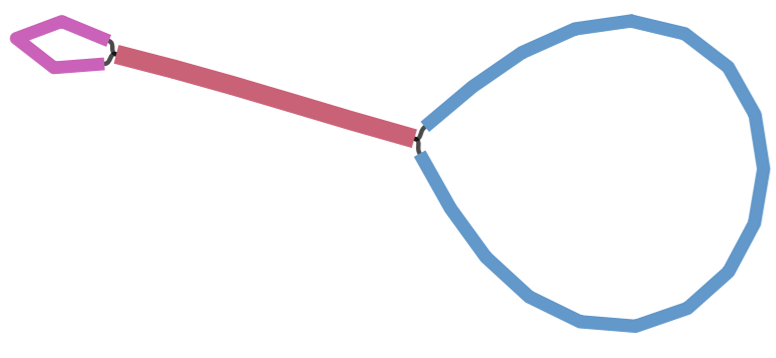
\includegraphics[width=1\linewidth]{Images/Amphoricarpus_bandage} \caption{Bandage visualization of contig structure of plastome assembly for Amphoricarpus autariatus. A complete plastome assembly should show this structure representing the 4 quadripartite regions of the plastome: a large circle representing the large single copy region, a small circle representing the small single copy region, and and a connecting line representing the two inverted repeat regions.}\label{fig:bandage}
\end{figure}

\hypertarget{running-geseq}{%
\subsubsection{Running GeSeq}\label{running-geseq}}

GeSeq (\protect\hyperlink{ref-Tillich2017}{Tillich et al., 2017}) is a web-based applicaion that was developed for the rapid and accurate annotation of organelle genomes, in particular chloroplast genomes. Complete circular plastome assemblies may be annotated using GeSeq (\protect\hyperlink{ref-Tillich2017}{Tillich et al., 2017}) and visualized using OGDraw at \url{https://chlorobox.mpimp-golm.mpg.de/geseq.html}.

\begin{figure}
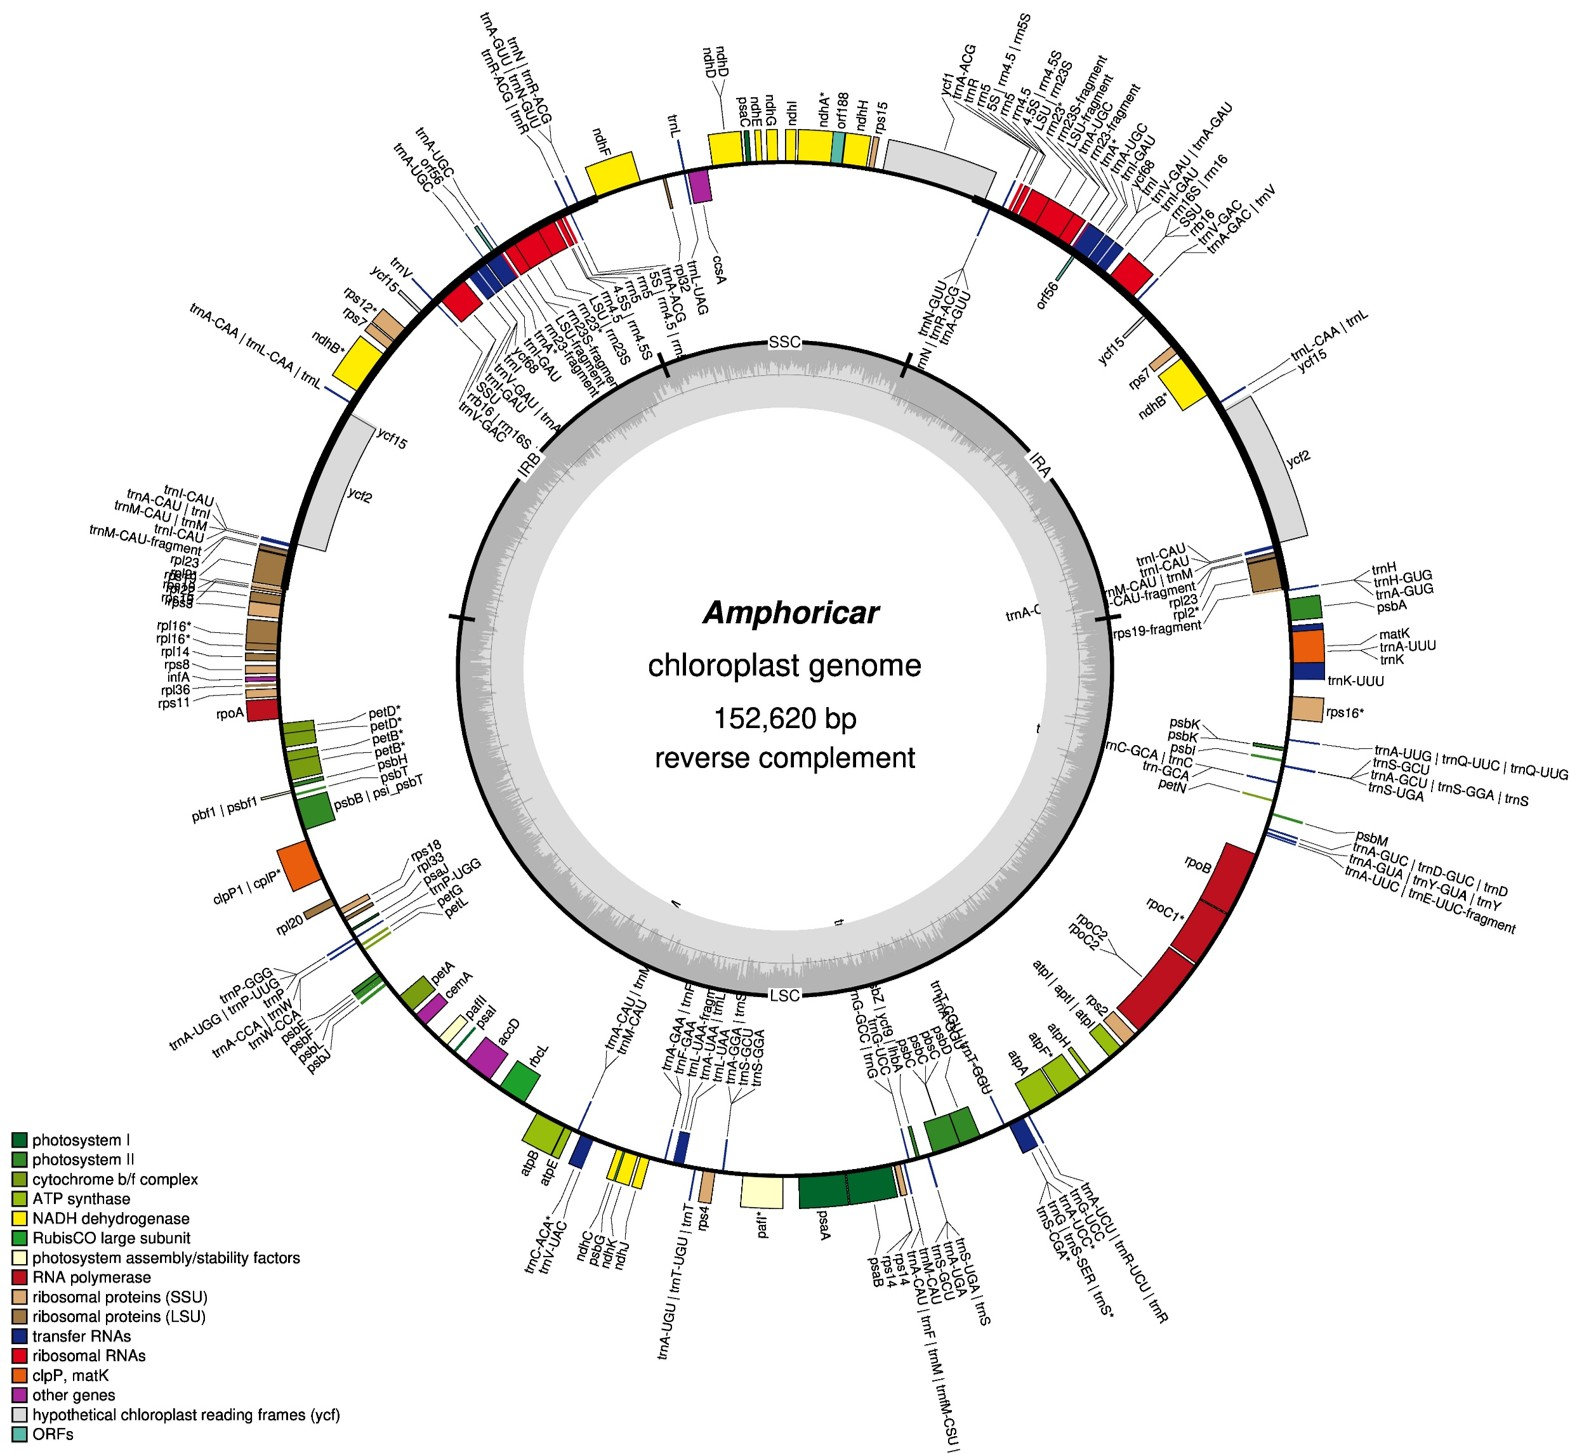
\includegraphics[width=1\linewidth]{Images/GeSeqJob-20240601-170716_Amphoricarpos_autariatus_OGDRAW} \caption{Annotated chloroplast of Amphoricarpos autariatus produced by OGDraw.}\label{fig:ogdraw}
\end{figure}

\hypertarget{generating-species-phylogenies}{%
\section{Generating Species Phylogenies}\label{generating-species-phylogenies}}

\hypertarget{identifying-ultra-conserved-elements-from-target-enriched-data}{%
\subsection{Identifying ultra-conserved elements from target-enriched data}\label{identifying-ultra-conserved-elements-from-target-enriched-data}}

PHYLUCE (\protect\hyperlink{ref-Faircloth2016}{Faircloth, 2016}) is a software that determines orthology from targeted loci/genes (e.g., from target-enrichment data). It is considered `ultra-conserved' compared to other orthology determination softwares (e.g., HybPiper) since it removes any loci that is considered paralogous. Other poeple use hybpiper blah blah , skip down to blah model selection section use your concatenated gene file.

\hypertarget{installing-phyluce}{%
\subsubsection{Installing Phyluce}\label{installing-phyluce}}

\begin{Shaded}
\begin{Highlighting}[]
\CommentTok{\#bash}
\ExtensionTok{conda}\NormalTok{ create }\AttributeTok{{-}{-}name}\NormalTok{ phyluce}
\ExtensionTok{conda}\NormalTok{ activate phyluce}
\ExtensionTok{conda}\NormalTok{ install bioconda::phyluce}
\end{Highlighting}
\end{Shaded}

\hypertarget{running-phyluce}{%
\subsubsection{Running PHYLUCE}\label{running-phyluce}}

\textbf{INPUT}

\begin{itemize}
\tightlist
\item
  contigs/*.fasta, folder containing all contig files (output from SPAdes)
\item
  datasets.conf, a file containing a list of species used in the analysis. Species names should be separated by ``\_``. When using this, you need to reference which species you want to refer to by indicating it with the `taxon-group' flag.
\item
  phyluce\_cos1061\_probes.fasta: the probe file with gene names and sequences from targeted genes.
\end{itemize}

NOTE: Make sure to change the file paths throughout and change the number of taxa to the appropriate number at each `--taxa' flag when needed.

\begin{Shaded}
\begin{Highlighting}[]
\CommentTok{\#bash}
\CommentTok{\#activate the conda environment}
\ExtensionTok{conda}\NormalTok{ activate phyluce}

\CommentTok{\# Create empty log folder}
\FunctionTok{mkdir}\NormalTok{ ./log}

\CommentTok{\# Generate *.lastz files for each contig from SPAdes.}
\ExtensionTok{python}\NormalTok{ /home/USER/miniconda3/envs/phyluce/bin/phyluce\_assembly\_match\_contigs\_to\_probes     }\AttributeTok{{-}{-}contigs}\NormalTok{ ./contigs     }\AttributeTok{{-}{-}probes}\NormalTok{ cos\_probes.fasta     }\AttributeTok{{-}{-}output}\NormalTok{ ./output     }\AttributeTok{{-}{-}log{-}path}\NormalTok{ ./log}

\CommentTok{\#Resulting files are *.lastz files in the ‘output’ folder. These files only need to be made once and are only probe–not species–specific.}

\CommentTok{\# Create empty output directory, in this case it is called ‘taxon{-}set{-}all’}
\FunctionTok{mkdir}\NormalTok{ ./taxon{-}set{-}all/}

\CommentTok{\#create the initial list of loci for each taxon}
\ExtensionTok{python}\NormalTok{ /home/USER/miniconda3/envs/phyluce/bin/phyluce\_assembly\_get\_match\_counts     }\AttributeTok{{-}{-}locus{-}db}\NormalTok{ ./output/probe.matches.sqlite     }\AttributeTok{{-}{-}taxon{-}list{-}config}\NormalTok{ datasets.conf     }\AttributeTok{{-}{-}taxon{-}group} \StringTok{\textquotesingle{}subset4\textquotesingle{}}     \AttributeTok{{-}{-}output}\NormalTok{ ./taxon{-}set{-}all/all.conf     }\AttributeTok{{-}{-}incomplete{-}matrix}     \AttributeTok{{-}{-}log{-}path}\NormalTok{ ./log}

\CommentTok{\# extract FASTA data that correspond to the loci in all{-}taxa{-}incomplete.conf}
\ExtensionTok{python}\NormalTok{ /home/USER/miniconda3/envs/phyluce/bin/phyluce\_assembly\_get\_fastas\_from\_match\_counts  }\AttributeTok{{-}{-}contigs}\NormalTok{ ./contigs   }\AttributeTok{{-}{-}locus{-}db}\NormalTok{ ./output/probe.matches.sqlite }\AttributeTok{{-}{-}match{-}count{-}output}\NormalTok{ ./taxon{-}set{-}all/all.conf }\AttributeTok{{-}{-}incomplete{-}matrix}\NormalTok{ ./taxon{-}set{-}all/all.incomplete }\AttributeTok{{-}{-}output}\NormalTok{ ./taxon{-}set{-}all/all.fasta }\AttributeTok{{-}{-}log{-}path}\NormalTok{ ./log}

\CommentTok{\# Explode the monolithic FASTA}
\ExtensionTok{python}\NormalTok{ /PATH/TO/miniconda3/envs/phyluce/bin/phyluce\_assembly\_explode\_get\_fastas\_file }\AttributeTok{{-}{-}input}\NormalTok{ ./taxon{-}set{-}all/all.fasta }\AttributeTok{{-}{-}output}\NormalTok{ exploded{-}fastas}

\CommentTok{\# Then run the below code to get stats}
\ControlFlowTok{for}\NormalTok{ i }\KeywordTok{in}\NormalTok{ exploded{-}fastas/}\PreprocessorTok{*}\NormalTok{.fasta}\KeywordTok{;}
\ControlFlowTok{do}
\ExtensionTok{python}\NormalTok{ /PATH/TO/miniconda3/envs/phyluce/bin/phyluce\_assembly\_get\_fasta\_lengths }\AttributeTok{{-}{-}input} \VariableTok{$i} \AttributeTok{{-}{-}csv}\KeywordTok{;}
\ControlFlowTok{done} \OperatorTok{\textgreater{}}\NormalTok{ fasta\_lengths.csv}
\CommentTok{\#the resulting csv has summary stats on the FASTAS}
\CommentTok{\#the column headers are: samples,contigs,total bp,mean length,95 CI length,min length,max length,median length,contigs \textgreater{}1kb}

\CommentTok{\# Alignment without internal trimming BUT does edge trim }
\CommentTok{\#CHANGE TAXON NUMBER}
\ExtensionTok{python}\NormalTok{ /PATH/TO/miniconda3/envs/phyluce/bin/phyluce\_align\_seqcap\_align }\AttributeTok{{-}{-}input}\NormalTok{ ./taxon{-}set{-}all/all.fasta  }\AttributeTok{{-}{-}output}\NormalTok{ ./taxon{-}set{-}all/mafft{-}nexus{-}trimmed/ }\AttributeTok{{-}{-}taxa}\NormalTok{ 11 }\AttributeTok{{-}{-}aligner}\NormalTok{ mafft }\AttributeTok{{-}{-}cores}\NormalTok{ 4 }\AttributeTok{{-}{-}incomplete{-}matrix} \AttributeTok{{-}{-}log{-}path}\NormalTok{ ./log}

\CommentTok{\# Get basic stats on the alignments  }
\ExtensionTok{python}\NormalTok{ /PATH/TO/miniconda3/envs/phyluce/bin/phyluce\_align\_get\_align\_summary\_data }\AttributeTok{{-}{-}alignments}\NormalTok{ ./taxon{-}set{-}all/mafft{-}nexus{-}trimmed/ }\AttributeTok{{-}{-}cores}\NormalTok{ 4 }\AttributeTok{{-}{-}log{-}path}\NormalTok{ ./log}

\CommentTok{\# Remove locus name from alignments   }
\ExtensionTok{python}\NormalTok{ /PATH/TO/miniconda3/envs/phyluce/bin/phyluce\_align\_remove\_locus\_name\_from\_files }\AttributeTok{{-}{-}alignments}\NormalTok{ ./taxon{-}set{-}all/mafft{-}nexus{-}trimmed/ }\AttributeTok{{-}{-}output}\NormalTok{ ./taxon{-}set{-}all/mafft{-}nexus{-}trimmed{-}clean/ }\AttributeTok{{-}{-}log{-}path}\NormalTok{ ./log}

\CommentTok{\# Generates individual gene matrix files that will be used for the pseudo{-}coalescent analysis}
\CommentTok{\#CHANGE TAXON NUMBER}
\ExtensionTok{python}\NormalTok{ /PATH/TO/miniconda3/envs/phyluce/bin/phyluce\_align\_get\_only\_loci\_with\_min\_taxa }\AttributeTok{{-}{-}alignments}\NormalTok{ ./taxon{-}set{-}all/mafft{-}nexus{-}trimmed{-}clean }\AttributeTok{{-}{-}taxa}\NormalTok{ 11 }\AttributeTok{{-}{-}percent}\NormalTok{ 0 }\AttributeTok{{-}{-}output}\NormalTok{ ./taxon{-}set{-}all/mafft{-}nexus{-}trimmed{-}clean{-}genes }\AttributeTok{{-}{-}cores}\NormalTok{ 4 }\AttributeTok{{-}{-}log{-}path}\NormalTok{ ./log}

\CommentTok{\# Build the total concatenated data matrix from the gene matrices}
\ExtensionTok{python}\NormalTok{ /PATH/TO/miniconda3/envs/phyluce/bin/phyluce\_align\_concatenate\_alignments }\AttributeTok{{-}{-}alignments}\NormalTok{ ./taxon{-}set{-}all/mafft{-}nexus{-}trimmed{-}clean{-}genes }\AttributeTok{{-}{-}output}\NormalTok{ ./taxon{-}set{-}all/mafft{-}nexus{-}trimmed{-}raxml }\AttributeTok{{-}{-}phylip} \AttributeTok{{-}{-}log{-}path}\NormalTok{ ./log}

\CommentTok{\# Converts nexus to phylip{-}relaxed file format}
\ExtensionTok{python}\NormalTok{ /PATH/TO/miniconda3/envs/phyluce/bin/phyluce\_align\_convert\_one\_align\_to\_another }\AttributeTok{{-}{-}alignments}\NormalTok{ ./taxon{-}set{-}all/mafft{-}nexus{-}trimmed{-}clean{-}genes }\AttributeTok{{-}{-}output}\NormalTok{ ./taxon{-}set{-}all/mafft{-}fasta }\AttributeTok{{-}{-}input{-}format}\NormalTok{ nexus }\AttributeTok{{-}{-}output{-}format}\NormalTok{ phylip{-}relaxed }\AttributeTok{{-}{-}cores}\NormalTok{ 1 }\AttributeTok{{-}{-}log{-}path}\NormalTok{ ./log}
\end{Highlighting}
\end{Shaded}

\textbf{OUTPUT}

\begin{itemize}
\tightlist
\item
  fasta\_lengths.csv, summary stats on all sequences
\item
  ./Exploded\_fastas/, folder containing unaligned sequence data used to generate the summary statistics (fasta\_lengths.csv)
\item
  ./Taxon\_set\_all/
\item
  all.conf, logs which taxa and genes were recovered with PHYLUCE
\item
  all.fasta, all gene sequences that matched the probe set for each taxon as a multifasta file
\item
  all.incomplete, lists all genes that did not match the probe set for each taxon
\item
  mafft-nexus-trimmed/, folder containing all aligned sequences without internal trimming BUT does edge trim
\item
  mafft-nexus-trimmed-clean/, folder similar to `mafft-nexus-trimmed/' but removed the locus name from the alignment
\item
  mafft-nexus-trimmed-clean-genes/, folder containing gene files that will be used for pseudo-coalescent analysis
\item
  mafft-nexus-trimmed-raxml/, folder containing the concatenated gene matrix of all genes and taxa along with a `charsets' file that will be used for model selection
\item
  mafft-fasta/, folder similar to `mafft-nexus-trimmed-raxml/' but has the files as phylip-relaxed instead of nexus
\end{itemize}

(Optional) Extracting data from the sqlite database produced by PHYLUCE
PHYLUCE produces a sqlite database that contains two tables: ``matches'' and ``match\_map''. ``matches'' contains which loci were recovered for each taxa, while ``match\_map'' has the name of the contig that matches each loci in each taxa. We can use the following commands to save these tables as csv files.

1 Nvigate to the PHYLUCE output/ folder. The sqlite file ( probe.matches.sqlite) should be there.
2 Open the file:
sqlite3 probe.matches.sqlite
3 ``sqlite\textgreater{}'' should be in the working line.
NOTE: With the code below, the ``sqlite\textgreater{}'' bit is the prompt, you don't need to type it down. Type one command at a time and hit enter.
+ sqlite\textgreater{} .headers on\\
+ sqlite\textgreater{} .mode csv
+ sqlite\textgreater{} .output matches.csv \#creates the first file
+ sqlite\textgreater{} SELECT * FROM matches; \#populate the file with the contents of the matches table
+sqlite\textgreater{} .output match\_map.csv \#creates the second file
+sqlite\textgreater{} SELECT * FROM match\_map; \#populate the file with the contents of the match\_map
+sqlite\textgreater{} .quit \#exits sqlite
4 Output: matches.csv and match\_map.csv. These files can be downloaded to get more stats on your PHYLUCE run.

\hypertarget{model-selection}{%
\subsection{Model Selection}\label{model-selection}}

These next few steps will detail how to run PartitionFinder (\protect\hyperlink{ref-Lanfear2016}{Lanfear et al., 2016}) to determine which evolutionary model best fits our data to then generate gene trees.

\hypertarget{installing-partitionfinder}{%
\subsubsection{Installing PartitionFinder}\label{installing-partitionfinder}}

Installation instructions can be found at www.robertlanfear.com/partitionfinder/tutorial.

\hypertarget{running-partitionfinder}{%
\subsubsection{Running PartitionFinder}\label{running-partitionfinder}}

\textbf{INPUT}

\begin{itemize}
\tightlist
\item
  *.phylip, tree file (output from Phyluce)
\item
  *.charsets, character set file (output from Phyluce)
\end{itemize}

Using the charsets file, create a configuration (.cfg) file with information about the matrix. You may use the following command to make this file.

\begin{Shaded}
\begin{Highlighting}[]
\CommentTok{\#bash}
\CommentTok{\#designate the input file. Change if needed}

\VariableTok{input\_file}\OperatorTok{=}\StringTok{"mafft{-}nexus{-}trimmed{-}raxml.charsets"} 
\CommentTok{\#designate the output file. Change if needed}

\VariableTok{output\_file}\OperatorTok{=}\StringTok{"partition\_finder.cfg"} 

\CommentTok{\# Start by writing the static part of the output}
\BuiltInTok{echo} \StringTok{"alignment = mafft{-}nexus{-}trimmed{-}raxml.phylip;"} \OperatorTok{\textgreater{}} \StringTok{"}\VariableTok{$output\_file}\StringTok{"} \CommentTok{\#Change the alignment name if needed}
\BuiltInTok{echo} \StringTok{"branchlengths = linked;"} \OperatorTok{\textgreater{}\textgreater{}} \StringTok{"}\VariableTok{$output\_file}\StringTok{"}
\BuiltInTok{echo} \StringTok{"models = all;"} \OperatorTok{\textgreater{}\textgreater{}} \StringTok{"}\VariableTok{$output\_file}\StringTok{"}
\BuiltInTok{echo} \StringTok{"model\_selection = AICc;"} \OperatorTok{\textgreater{}\textgreater{}} \StringTok{"}\VariableTok{$output\_file}\StringTok{"}
\BuiltInTok{echo} \StringTok{"[data\_blocks]"} \OperatorTok{\textgreater{}\textgreater{}} \StringTok{"}\VariableTok{$output\_file}\StringTok{"}

\CommentTok{\# Process the input file to extract and format the charset lines}
\FunctionTok{awk} \StringTok{\textquotesingle{}/\^{}charset/ \{}
\StringTok{    split($2, a, "=");}
\StringTok{    gsub(/charset |\textbackslash{}.nexus|\textquotesingle{}}\DataTypeTok{\textbackslash{}\textquotesingle{}}\StringTok{\textquotesingle{}/, "", $2);  \# Remove charset, .nexus, and single quotes}
\StringTok{    print $2 " = " $4;}
\StringTok{\}\textquotesingle{}} \StringTok{"}\VariableTok{$input\_file}\StringTok{"} \OperatorTok{\textgreater{}\textgreater{}} \StringTok{"}\VariableTok{$output\_file}\StringTok{"}

\CommentTok{\# Add the [schemes] section to the output}
\BuiltInTok{echo} \StringTok{"[schemes]"} \OperatorTok{\textgreater{}\textgreater{}} \StringTok{"}\VariableTok{$output\_file}\StringTok{"}
\BuiltInTok{echo} \StringTok{"search = rcluster;"} \OperatorTok{\textgreater{}\textgreater{}} \StringTok{"}\VariableTok{$output\_file}\StringTok{"}
\end{Highlighting}
\end{Shaded}

Using the newly made .cfg file, run the following code:

\begin{Shaded}
\begin{Highlighting}[]
\CommentTok{\#bash}
\ExtensionTok{/PATH/TO/PartitionFinder.py}\NormalTok{ /PATH/TO/partition\_finder.cfg }\AttributeTok{{-}{-}raxml} \AttributeTok{{-}{-}rcluster{-}max}\NormalTok{ 100 }\AttributeTok{{-}{-}no{-}ml{-}tree}
\end{Highlighting}
\end{Shaded}

\textbf{OUTPUT}

\begin{itemize}
\tightlist
\item
  log.txt, log file
\item
  analysis/best\_scheme.txt, file listing loci along with their corresponding best model.
\end{itemize}

\hypertarget{concatenated-phylogeny}{%
\subsection{Concatenated Phylogeny}\label{concatenated-phylogeny}}

When analyzing target-enriched sequencing data for phylogenetic analyses, multiple approaches may be implemented. For a concatenated approach all gene sequences are combined into a single matrix. This method assumes that all trees share the same evolutionary history, and therefore may not always be ideal for ancient divergences where gene trees are highly divergent. This tutorial presents instructions for a concatenated phylogeny using RAxML (\protect\hyperlink{ref-Stamatakis2014}{Stamatakis, 2014}), a maximum likelihood phylogenetic inference tool. Phylogenetic trees may be visualized by an array of tools, eg. FigTree (\url{http://tree.bio.ed.ac.uk/software/figtree/}).

\hypertarget{installing-raxml}{%
\subsubsection{Installing RAxML}\label{installing-raxml}}

Installation instructions can be found at \url{https://cme.h-its.org/exelixis/web/software/raxml/cluster.html}.

\hypertarget{running-raxml-on-a-concatenated-matrix}{%
\subsubsection{Running RAxML on a concatenated matrix}\label{running-raxml-on-a-concatenated-matrix}}

\textbf{INPUT}

\begin{itemize}
\tightlist
\item
  *.phylip, tree file (output from Phyluce)
\end{itemize}

Note: Change the -m function depending on the best fitting model (GTR model: GTRCAT; GTR+G model: GTRGAMMA; GTR+I+G model: GTRGAMMAI).

\begin{Shaded}
\begin{Highlighting}[]
\CommentTok{\#bash}
\ExtensionTok{/PATH/TO/raxmlHPC{-}PTHREADS{-}SSE3} \AttributeTok{{-}T} \VariableTok{$SLURM\_CPUS\_PER\_TASK} \AttributeTok{{-}f}\NormalTok{ a }\AttributeTok{{-}p}\NormalTok{ 12345 }\AttributeTok{{-}x}\NormalTok{ 12345 }\AttributeTok{{-}m}\NormalTok{ GTRGAMMAI }\AttributeTok{{-}\#}\NormalTok{ 100 }\AttributeTok{{-}s}\NormalTok{ /PATH/TO/mafft{-}nexus{-}trimmed{-}raxml.phylip }\AttributeTok{{-}n}\NormalTok{ out}
\end{Highlighting}
\end{Shaded}

\textbf{OUTPUT}

\emph{RAxML\_bipartitionsBranchLabels.out
}RAxML\_bootstrap.out
\emph{RAxML\_info.out
}RAxML\_bestTree.out
*RAxML\_bipartitions.out

\hypertarget{installing-figtree}{%
\subsubsection{Installing FigTree}\label{installing-figtree}}

Installation instructions can be found at \url{https://evomics.org/resources/software/molecular-evolution-software/figtree/}.

\textbf{INPUT}

\begin{itemize}
\tightlist
\item
  RAxML\_bipartitionsBranchLabels.out, output from RAxML
\end{itemize}

\textbf{OUTPUT}

\begin{itemize}
\tightlist
\item
  visualizations may be exported in multiple formats
\end{itemize}

\begin{figure}

\includegraphics[width=1\linewidth]{Images/concat.raxml} \caption{Phylogenetic tree produced from RAxML analysis on a concatenated matrix visualized using FigTree.}(\#fig:concat_tree)
\end{figure}

\hypertarget{coalescent-based-phylogeny}{%
\subsection{Coalescent-based Phylogeny}\label{coalescent-based-phylogeny}}

In contrast to a concatenated approach, a coalescent phylogenetic approach analyzes individual gene tree, accounting for the fact that different genes may have different evolutionary histories. This method may be better suited for resolving phylogenetic relationships in the presence of incomplete lineage sorting and hybridization, but is more computationally demanding than concatenated methods. One method to generate a coalescent phylogeny is by using Astral-III (\protect\hyperlink{ref-Zhang2018}{Zhang et al., 2018}) on a suite of RAxML (\protect\hyperlink{ref-Stamatakis2014}{Stamatakis, 2014}) gene trees constructed under different models. Resulting phylogenetic trees may be visualized by an array of tools, eg. FigTree (\url{http://tree.bio.ed.ac.uk/software/figtree/}).

\hypertarget{installing-raxml-1}{%
\subsubsection{Installing RAxML}\label{installing-raxml-1}}

Installation instructions can be found at \url{https://cme.h-its.org/exelixis/web/software/raxml/cluster.html}.

\hypertarget{running-raxml-for-coalescent-analyses}{%
\subsubsection{Running RAxML for coalescent analyses}\label{running-raxml-for-coalescent-analyses}}

When running RAxmL for a pseudo-coalescent (hereafter referred to as ``ASTRAL'') analysis, you should separate the individual loci by their most appropriate model as indicated by the results of PartitionFinder and run each loci separately.

\textbf{INPUT}

\begin{itemize}
\tightlist
\item
  uce-*.nexus, individual loci file in nexus format (output from Phyluce)
\item
  analysis/best\_scheme.txt, file denoting the best model for each loci (output from Phyluce)
\end{itemize}

To organize all loci files into new directories pertaining to each model type, you can use the following code. In this code, loci files (eg. uce-*.nexus) will be moved into folders labeled ``batch\_exports''.

\begin{Shaded}
\begin{Highlighting}[]
\CommentTok{\#bash}
\CommentTok{\#make folders of each model type in main working directory}
\FunctionTok{mkdir}\NormalTok{ astral\_raxml}
\BuiltInTok{cd}\NormalTok{ astral\_raxml}

\FunctionTok{mkdir}\NormalTok{ bestTree}
\FunctionTok{mkdir}\NormalTok{ bootTree}
\FunctionTok{mkdir}\NormalTok{ Astral\_try}

\FunctionTok{mkdir}\NormalTok{ GTR}
\FunctionTok{mkdir}\NormalTok{ GTRG}
\FunctionTok{mkdir}\NormalTok{ GTRIG}
\BuiltInTok{cd}\NormalTok{ GTR}
\FunctionTok{mkdir}\NormalTok{ GTR\_batch\_exports}
\FunctionTok{mkdir}\NormalTok{ output}
\BuiltInTok{cd}\NormalTok{ ../GTRG}
\FunctionTok{mkdir}\NormalTok{ GTRG\_batch\_exports}
\FunctionTok{mkdir}\NormalTok{ output}
\BuiltInTok{cd}\NormalTok{ ../GTRIG}
\FunctionTok{mkdir}\NormalTok{ GTRIG\_batch\_exports}
\FunctionTok{mkdir}\NormalTok{ output}

\CommentTok{\#edit the best\_scheme.txt file to be used for designating loci files to proper model folder}
\FunctionTok{tail} \AttributeTok{{-}n}\NormalTok{ +22 best\_scheme.txt}\KeywordTok{|} \FunctionTok{sed} \AttributeTok{{-}n} \StringTok{\textquotesingle{}/\^{}$/q;p\textquotesingle{}} \OperatorTok{\textgreater{}}\NormalTok{ best\_scheme\_uce\_table.txt}
\end{Highlighting}
\end{Shaded}

Move each loci folder to its designated model folder using the following R code. Change the uce location paths to match your own directory organization.

\begin{Shaded}
\begin{Highlighting}[]
\CommentTok{\#R}

\FunctionTok{df} \OperatorTok{\textless{}}\NormalTok{{-} read.table}\ErrorTok{(}\FunctionTok{file}\NormalTok{ = }\StringTok{"best\_scheme\_uce\_table.txt"}\NormalTok{, header = TRUE, sep = }\StringTok{"|"}\NormalTok{, na.strings = }\StringTok{""}\NormalTok{, comment.char = }\StringTok{""}\NormalTok{, quote = }\StringTok{"}\DataTypeTok{\textbackslash{}"}\StringTok{"}\NormalTok{, fill = FALSE, nrows = 200000}\KeywordTok{)}

\ExtensionTok{df}\VariableTok{$Best}\ExtensionTok{.Model} \OperatorTok{\textless{}}\NormalTok{{-} gsub}\ErrorTok{(}\StringTok{" "}\ExtensionTok{,} \StringTok{""}\NormalTok{, df}\VariableTok{$Best}\NormalTok{.Model, fixed = TRUE}\KeywordTok{)}
\ExtensionTok{df}\VariableTok{$Partition}\ExtensionTok{.names} \OperatorTok{\textless{}}\NormalTok{{-} gsub}\ErrorTok{(}\StringTok{" "}\ExtensionTok{,} \StringTok{""}\NormalTok{, df}\VariableTok{$Partition}\NormalTok{.names, fixed = TRUE}\KeywordTok{)}

\ExtensionTok{GTR} \OperatorTok{\textless{}}\NormalTok{{-} c}\ErrorTok{(}\ExtensionTok{unlist}\ErrorTok{(}\ExtensionTok{strsplit}\ErrorTok{(}\ExtensionTok{df}\VariableTok{$Partition}\ExtensionTok{.names[which}\ErrorTok{(}\ExtensionTok{df}\VariableTok{$Best}\ExtensionTok{.Model}\NormalTok{ == }\StringTok{"GTR"}\KeywordTok{)}\ExtensionTok{],}\StringTok{","}\KeywordTok{)))}
\ExtensionTok{GTRG} \OperatorTok{\textless{}}\NormalTok{{-} c}\ErrorTok{(}\ExtensionTok{unlist}\ErrorTok{(}\ExtensionTok{strsplit}\ErrorTok{(}\ExtensionTok{df}\VariableTok{$Partition}\ExtensionTok{.names[which}\ErrorTok{(}\ExtensionTok{df}\VariableTok{$Best}\ExtensionTok{.Model}\NormalTok{ == }\StringTok{"GTR+G"}\KeywordTok{)}\ExtensionTok{],}\StringTok{","}\KeywordTok{)))}
\ExtensionTok{GTRIG} \OperatorTok{\textless{}}\NormalTok{{-} c}\ErrorTok{(}\ExtensionTok{unlist}\ErrorTok{(}\ExtensionTok{strsplit}\ErrorTok{(}\ExtensionTok{df}\VariableTok{$Partition}\ExtensionTok{.names[which}\ErrorTok{(}\ExtensionTok{df}\VariableTok{$Best}\ExtensionTok{.Model}\NormalTok{ == }\StringTok{"GTR+I+G"}\KeywordTok{)}\ExtensionTok{],}\StringTok{","}\KeywordTok{)))}

\ExtensionTok{model\_GTR} \OperatorTok{\textless{}}\NormalTok{{-} cbind}\ErrorTok{(}\ExtensionTok{GTR,}\NormalTok{ rep}\ErrorTok{(}\StringTok{"GTR"}\ExtensionTok{,}\NormalTok{ n= length}\ErrorTok{(}\ExtensionTok{GTR}\KeywordTok{)))}
\ExtensionTok{model\_GTRG} \OperatorTok{\textless{}}\NormalTok{{-} cbind}\ErrorTok{(}\ExtensionTok{GTRG,}\NormalTok{ rep}\ErrorTok{(}\StringTok{"GTRG"}\ExtensionTok{,}\NormalTok{ n= length}\ErrorTok{(}\ExtensionTok{GTRG}\KeywordTok{)))}
\ExtensionTok{model\_GTRIG} \OperatorTok{\textless{}}\NormalTok{{-} cbind}\ErrorTok{(}\ExtensionTok{GTRIG,}\NormalTok{ rep}\ErrorTok{(}\StringTok{"GTRIG"}\ExtensionTok{,}\NormalTok{ n= length}\ErrorTok{(}\ExtensionTok{GTRIG}\KeywordTok{)))}

\ExtensionTok{model\_df} \OperatorTok{\textless{}}\NormalTok{{-} as.data.frame}\ErrorTok{(}\ExtensionTok{rbind}\ErrorTok{(}\ExtensionTok{model\_GTR,}\NormalTok{ model\_GTRG, model\_GTRIG}\KeywordTok{))}
\ExtensionTok{colnames}\ErrorTok{(}\ExtensionTok{model\_df}\KeywordTok{)} \OperatorTok{\textless{}}\NormalTok{{-} }\ExtensionTok{c}\ErrorTok{(}\StringTok{"uce"}\ExtensionTok{,} \StringTok{"model"}\KeywordTok{)}


\ExtensionTok{uce\_original\_location} \OperatorTok{\textless{}}\NormalTok{{-} }\StringTok{"/PATH/TO/taxon{-}set{-}all/mafft{-}nexus{-}trimmed{-}clean{-}100p/"}
\ExtensionTok{uce\_model\_location} \OperatorTok{\textless{}}\NormalTok{{-} }\StringTok{"/PATH/TO/astral\_raxml/"}
\ExtensionTok{files} \OperatorTok{\textless{}}\NormalTok{{-} list.files}\ErrorTok{(}\ExtensionTok{uce\_original\_location}\KeywordTok{)}

\ControlFlowTok{for}\KeywordTok{(}\ExtensionTok{i}\NormalTok{ in 1:length}\ErrorTok{(}\ExtensionTok{files}\KeywordTok{))} \KeywordTok{\{}
  
  \ExtensionTok{file\_name} \OperatorTok{\textless{}}\NormalTok{{-} files}\PreprocessorTok{[}\SpecialStringTok{i}\PreprocessorTok{]}
  \ExtensionTok{file\_uce} \OperatorTok{\textless{}}\NormalTok{{-} gsub}\ErrorTok{(}\StringTok{".nexus"}\ExtensionTok{,} \StringTok{""}\NormalTok{, file\_name}\KeywordTok{)}
  \ExtensionTok{file\_model} \OperatorTok{\textless{}}\NormalTok{{-} model\_df}\VariableTok{$model}\NormalTok{[which}\ErrorTok{(}\ExtensionTok{model\_df}\VariableTok{$uce}\NormalTok{ \%in\% file\_uce}\KeywordTok{)}\ExtensionTok{]}
  \ExtensionTok{file.copy}\ErrorTok{(}\ExtensionTok{from}\NormalTok{ = paste}\ErrorTok{(}\ExtensionTok{uce\_original\_location,}\NormalTok{ file\_name, sep = }\StringTok{""}\KeywordTok{)}\ExtensionTok{,to}\NormalTok{ = paste}\ErrorTok{(}\ExtensionTok{uce\_model\_location,}\NormalTok{ file\_model, }\StringTok{"/"}\NormalTok{, file\_model, }\StringTok{"\_batch\_exports"}\NormalTok{, sep = }\StringTok{""}\KeywordTok{))}
  
\KeywordTok{\}}
\end{Highlighting}
\end{Shaded}

Once all the gene files ARE in their appropriate model choice's batch\_export/ folder, the file type and ending will need to be changed from .nexus to .fasta. This can be doe using the tool ElConcatenero (\url{https://github.com/ODiogoSilva/TriFusion}) using the following code.

\begin{Shaded}
\begin{Highlighting}[]
\CommentTok{\#bash}
\ExtensionTok{python}\NormalTok{ /home/USER/ElConcatenero/ElConcatenero.py }\AttributeTok{{-}c} \AttributeTok{{-}if}\NormalTok{ nexus }\AttributeTok{{-}of}\NormalTok{ fasta }\AttributeTok{{-}in} \PreprocessorTok{*}\NormalTok{.nexus}
\end{Highlighting}
\end{Shaded}

RAxML can then be run on the individual, aligned gene files in a loop. The -m flag will need to be adjusted depending on the best fitting model (GTR model: GTRCAT; GTR+G model: GTRGAMMA; GTR+I+G model: GTRGAMMAI).

\begin{Shaded}
\begin{Highlighting}[]
\CommentTok{\#bash}
\VariableTok{DIR\_I}\OperatorTok{=}\NormalTok{/PATH/TO/astral\_raxml/GTR/batch\_exports/}\PreprocessorTok{*}

\ControlFlowTok{for}\NormalTok{ f }\KeywordTok{in} \VariableTok{$DIR\_I}
\ControlFlowTok{do}
\BuiltInTok{echo} \StringTok{"Processing }\VariableTok{$f}\StringTok{"}
\VariableTok{file\_name}\OperatorTok{=}\VariableTok{$(}\FunctionTok{basename} \VariableTok{$f)}
\ExtensionTok{/PATH/TO/raxmlHPC{-}PTHREADS{-}SSE3} \AttributeTok{{-}T}\NormalTok{ 4 }\AttributeTok{{-}f}\NormalTok{ a }\AttributeTok{{-}p}\NormalTok{ 12345 }\AttributeTok{{-}x}\NormalTok{ 12345 }\AttributeTok{{-}m}\NormalTok{ GTRCAT }\AttributeTok{{-}\#}\NormalTok{ 100 }\AttributeTok{{-}s} \VariableTok{$f} \AttributeTok{{-}n} \VariableTok{$file\_name} \AttributeTok{{-}w}\NormalTok{ /PATH/TO/astral\_raxml/GTR/output}
\ControlFlowTok{done}
\end{Highlighting}
\end{Shaded}

\textbf{OUTPUT}

\begin{itemize}
\tightlist
\item
  /output/RAxML\_bootstrap*, bootstrap files for each model type
\item
  /output/RAxML\_bestTree*, best tree files for each model type
\end{itemize}

Output from these RAxML (\protect\hyperlink{ref-Stamatakis2014}{Stamatakis, 2014}) analyses will be used as input for the Astral-III (\protect\hyperlink{ref-Zhang2018}{Zhang et al., 2018}) analysis.

\hypertarget{installing-astral-iii}{%
\subsubsection{Installing ASTRAL-III}\label{installing-astral-iii}}

Installation instructions can be found at \url{https://github.com/smirarab/ASTRAL}.

\hypertarget{running-astral-iii}{%
\subsubsection{Running ASTRAL-III}\label{running-astral-iii}}

\textbf{INPUT}

\begin{itemize}
\tightlist
\item
  RAxML\_bestTree*, tree files (output from RAxML)
\item
  RAxML\_bootstrap*, bootstrap files (output from RAxML)
\end{itemize}

After the output files are produced from RAxML, copy the RAxML\_bestTree* and RAxML\_bootstrap* files into their own folders. The file endings will then need to be changed and they will need to be concatenated. The following code may be used to prepare files for the ASTRAL analysis.

\begin{Shaded}
\begin{Highlighting}[]
\CommentTok{\#bash}
\CommentTok{\#make new folders}
\BuiltInTok{cd}\NormalTok{ /PATH/TO/astral\_raxml/}
\FunctionTok{mkdir}\NormalTok{ bestTree}
\FunctionTok{mkdir}\NormalTok{ bootTree}

\CommentTok{\#copy files to new folders}
\FunctionTok{cp}\NormalTok{ /PATH/TO/GTR/output/RAxML\_bootstrap}\PreprocessorTok{*}\NormalTok{ ./bootTree/}
\FunctionTok{cp}\NormalTok{ /PATH/TO/GTR/output/RAxML\_bestTree}\PreprocessorTok{*}\NormalTok{ ./bestTree/}

\CommentTok{\#change fasta extension to .tre extension}
\BuiltInTok{cd}\NormalTok{ bestTree}
\ControlFlowTok{for}\NormalTok{ f }\KeywordTok{in} \PreprocessorTok{*}\NormalTok{.fasta}\KeywordTok{;} \ControlFlowTok{do}
\FunctionTok{mv} \AttributeTok{{-}{-}} \StringTok{"}\VariableTok{$f}\StringTok{"} \StringTok{"}\VariableTok{$\{f}\OperatorTok{\%}\NormalTok{.fasta}\VariableTok{\}}\StringTok{.tre"}
\ControlFlowTok{done}
\BuiltInTok{cd}\NormalTok{ bootTree}
\ControlFlowTok{for}\NormalTok{ f }\KeywordTok{in} \PreprocessorTok{*}\NormalTok{.fasta}\KeywordTok{;} \ControlFlowTok{do}
\FunctionTok{mv} \AttributeTok{{-}{-}} \StringTok{"}\VariableTok{$f}\StringTok{"} \StringTok{"}\VariableTok{$\{f}\OperatorTok{\%}\NormalTok{.fasta}\VariableTok{\}}\StringTok{.tre"}
\ControlFlowTok{done}

\CommentTok{\#concatenate the .tre files}
\BuiltInTok{cd}\NormalTok{ bestTree}
\FunctionTok{cat}\NormalTok{ RAxML\_bestTree}\PreprocessorTok{*} \OperatorTok{\textgreater{}}\NormalTok{ concat\_best.tre }

\CommentTok{\#make a new folder named Astral and copy the concatenated best tree file into it}
\BuiltInTok{cd}\NormalTok{ /PATH/TO/astral\_raxml/}
\FunctionTok{mkdir}\NormalTok{ Astral\_try}
\BuiltInTok{cd}\NormalTok{ Astral\_try}
\FunctionTok{cp}\NormalTok{ ../bestTree/concat\_best.tre .}
\end{Highlighting}
\end{Shaded}

(Optional) We have stopped doing bootstrap analyses since the creators of ASTRAL-III said that LPP support values are more reliable than bootstrap, but the code is provided if you would like to do it. If you are running a bootstrap analysis, you also need to make a bs-files file which designates where the RAxML\_bootstrap*.tre files are (e.g., bootTree/).

\begin{Shaded}
\begin{Highlighting}[]
\CommentTok{\#example bs\_files}
\ExtensionTok{/PATH/TO/astral\_raxml/bootTree/RAxML\_bootstrap.uce{-}1000.tre}
\ExtensionTok{/PATH/TO/astral\_raxml/bootTree/RAxML\_bootstrap.uce{-}1005.tre}
\ExtensionTok{/PATH/TO/astral\_raxml/bootTree/RAxML\_bootstrap.uce{-}1007.tre}
\ExtensionTok{/PATH/TO/astral\_raxml/bootTree/RAxML\_bootstrap.uce{-}1008.tre}
\CommentTok{\# remaining bootstrap file locations}
\end{Highlighting}
\end{Shaded}

Code to make this bs-files is below.

\begin{Shaded}
\begin{Highlighting}[]
\CommentTok{\#bash}
\BuiltInTok{cd}\NormalTok{ /PATH/TO/astral\_raxml/bootTree/}
\FunctionTok{ls} \PreprocessorTok{*}\NormalTok{.tre }\OperatorTok{\textgreater{}}\NormalTok{ bs{-}files}
\BuiltInTok{pwd} \CommentTok{\#copy the directory!}
\FunctionTok{sed} \AttributeTok{{-}i} \StringTok{\textquotesingle{}s\textbackslash{}RAxML\textbackslash{}==/PATH/TO/astral\_raxml/bootTree/==RAxML\textbackslash{}g\textquotesingle{}}\NormalTok{ bs{-}files }\CommentTok{\#paste your working directory where it is highlighted!}
\FunctionTok{mv}\NormalTok{ bs{-}files ../Astral\_try/}
\end{Highlighting}
\end{Shaded}

ASTRAL-III can now be run with the following code:

\begin{Shaded}
\begin{Highlighting}[]
\CommentTok{\#bash}
\CommentTok{\#Run ASTRAL}
\ExtensionTok{java} \AttributeTok{{-}jar}\NormalTok{ /PATH/TO/ASTRAL/astral.5.7.3.jar  }\AttributeTok{{-}i}\NormalTok{ concat\_best.tre }\AttributeTok{{-}o}\NormalTok{ Astral\_best.tre }\DecValTok{2}\OperatorTok{\textgreater{}}\NormalTok{ astral\_best.log}

\CommentTok{\#Generate LPP values}
\ExtensionTok{java} \AttributeTok{{-}jar}\NormalTok{ /PATH/TO/ASTRAL/astral.5.7.3.jar  }\AttributeTok{{-}q}\NormalTok{ Astral\_best.tre  }\AttributeTok{{-}i}\NormalTok{ concat\_best.tre }\AttributeTok{{-}o}\NormalTok{ Astral\_lpp.tre }\DecValTok{2}\OperatorTok{\textgreater{}}\NormalTok{ astral\_lpp.log}

\CommentTok{\#Get bootstrap values (optional)}
\ExtensionTok{java} \AttributeTok{{-}jar}\NormalTok{ /PATH/TO/ASTRAL/astral.5.7.3.jar  }\AttributeTok{{-}i}\NormalTok{ concat\_best.tre }\AttributeTok{{-}b}\NormalTok{ bs{-}files }\AttributeTok{{-}o}\NormalTok{ Astral\_bootcount.tre }\DecValTok{2}\OperatorTok{\textgreater{}}\NormalTok{ astral\_bootcount.log}
\end{Highlighting}
\end{Shaded}

**OUTPUT

\begin{itemize}
\tightlist
\item
  *.log, log file
\item
  Astral.lpp.tre, final tree with LPP support values.
\end{itemize}

\hypertarget{installing-figtree-1}{%
\subsubsection{Installing FigTree}\label{installing-figtree-1}}

Installation instructions can be found at \url{https://evomics.org/resources/software/molecular-evolution-software/figtree/}.

\textbf{INPUT}

\begin{itemize}
\tightlist
\item
  Astral.lpp.tre, output from ASTRAL-III
\end{itemize}

\textbf{OUTPUT}

\begin{itemize}
\tightlist
\item
  visualizations may be exported in multiple formats
\end{itemize}

\begin{figure}

\includegraphics[width=1\linewidth]{Images/astral_tree} \caption{Phylogenetic tree produced from ASTRAL-III analysis visualized using FigTree.}(\#fig:astral_tree)
\end{figure}

\hypertarget{orthology-based-phylogeny}{%
\subsection{Orthology-based Phylogeny}\label{orthology-based-phylogeny}}

Another tool for generating phylogenetic trees within a coalescent framework is OrthoFinder (\protect\hyperlink{ref-Emms2019}{Emms and Kelly, 2019}). This program identifies orthogroups, infers rooted trees for all orthogroups, identifies gene duplication events, and infers a rooted species tree.

\hypertarget{installing-orthofinder}{%
\subsubsection{Installing OrthoFinder}\label{installing-orthofinder}}

\begin{Shaded}
\begin{Highlighting}[]
\CommentTok{\#bash}
\CommentTok{\# Install program with Bioconda}
\ExtensionTok{conda}\NormalTok{ create }\AttributeTok{{-}{-}name}\NormalTok{ orthofinder}
\ExtensionTok{conda}\NormalTok{ activate orthofinder}
\ExtensionTok{conda}\NormalTok{ install }\AttributeTok{{-}c}\NormalTok{ bioconda orthofinder}
\end{Highlighting}
\end{Shaded}

\hypertarget{running-orthofinder}{%
\subsubsection{Running OrthoFinder}\label{running-orthofinder}}

\textbf{INPUT}

\begin{itemize}
\tightlist
\item
  *.pep, peptide files
\end{itemize}

\begin{Shaded}
\begin{Highlighting}[]
\CommentTok{\#bash}
\ExtensionTok{/PATH/TO/OrthoFinder\_source/orthofinder.py} \AttributeTok{{-}f}\NormalTok{ ./pep/ }\AttributeTok{{-}t}\NormalTok{ 64 }\AttributeTok{{-}a}\NormalTok{ 16 }\AttributeTok{{-}M}\NormalTok{ msa }\AttributeTok{{-}T}\NormalTok{ raxml}
\end{Highlighting}
\end{Shaded}

\textbf{OUTPUT}

\begin{itemize}
\tightlist
\item
  SpeciesTree\_rooted.txt: rooted tree file
\end{itemize}

Refer to \url{https://davidemms.github.io/orthofinder_tutorials/exploring-orthofinders-results.html} for more detailed description of results.

\hypertarget{chloroplast-phylogeny}{%
\subsection{Chloroplast Phylogeny}\label{chloroplast-phylogeny}}

Phylogenetic trees from chloroplast sequencing data can be generated in a number of different ways. This tutorial will describe a method for plastome phylogenetic reconstruction using target-enriched sequencing data. As mentioned above in the plastome assembly section, there will often not be enough off-target sequence data for complete organellar assembly.

\hypertarget{installing-bowtie2-samtools-bcftools-seqtk}{%
\subsubsection{Installing Bowtie2, Samtools, BCFtools, seqtk}\label{installing-bowtie2-samtools-bcftools-seqtk}}

\begin{Shaded}
\begin{Highlighting}[]
\CommentTok{\#bash}
\CommentTok{\# Install program with Bioconda}
\ExtensionTok{conda}\NormalTok{ create }\AttributeTok{{-}{-}name}\NormalTok{ mapping}
\ExtensionTok{conda}\NormalTok{ activate mapping}
\ExtensionTok{conda}\NormalTok{ install bioconda::bowtie2}
\ExtensionTok{conda}\NormalTok{ install bioconda::samtools}
\ExtensionTok{conda}\NormalTok{ install bioconda::bcftools}
\ExtensionTok{conda}\NormalTok{ install bioconda::seqtk}
\end{Highlighting}
\end{Shaded}

\textbf{INPUT}

\begin{itemize}
\tightlist
\item
  *.tp.fastq, the trimmed sequence data
\end{itemize}

\hypertarget{running-bowtie2-samtools-bcftools-seqtk}{%
\subsubsection{Running Bowtie2, Samtools, BCFtools, seqtk}\label{running-bowtie2-samtools-bcftools-seqtk}}

This tutorial will describe a process of mapping off-target sequence reads to a reference plastome in order to create consensus sequences which may then be aligned and used as input for phylogenetic analyses.

\textbf{INPUT}

\begin{itemize}
\tightlist
\item
  reference.fasta, a reference plastome can be downloaded from GenBank or used from previous GetOrganelle analyses
\item
  *.tp.fastq, the trimmed sequence data for all samples
\end{itemize}

First, a reference database will need to be constructed using Bowtie2. This can be done using the following code:

\begin{Shaded}
\begin{Highlighting}[]
\CommentTok{\#bash}
\ExtensionTok{conda}\NormalTok{ activate mapping}

\ExtensionTok{bowtie2{-}build}\NormalTok{ reference\_plastome.fasta reference\_plastome}
\end{Highlighting}
\end{Shaded}

After a reference database has been built, the paired end target-enriched sequence reads may be mapped on to the reference plastome. To do this in a loop with all reads with file endings ``\_1\_tp.fastq'' and ``\_2\_tp.fastq'', use the following code:

\begin{Shaded}
\begin{Highlighting}[]
\CommentTok{\#bash}
\ExtensionTok{conda}\NormalTok{ activate mapping}

\CommentTok{\#in your working directory, make folders for output of this pipeline}
\FunctionTok{mkdir}\NormalTok{ sam\_files}
\FunctionTok{mkdir}\NormalTok{ bam\_files}
\FunctionTok{mkdir}\NormalTok{ fastq}
\FunctionTok{mkdir}\NormalTok{ consensus\_fastas}

\CommentTok{\#run the pipeline in a loop on all paired files}
\ControlFlowTok{for}\NormalTok{ fileR1 }\KeywordTok{in} \PreprocessorTok{*}\NormalTok{\_1\_tp.fastq}
\ControlFlowTok{do}
\VariableTok{fileR2}\OperatorTok{=}\KeywordTok{\textasciigrave{}}\BuiltInTok{echo} \VariableTok{$\{fileR1\}} \KeywordTok{|} \FunctionTok{sed} \StringTok{\textquotesingle{}s/\_1\_/\_2\_/\textquotesingle{}}\KeywordTok{\textasciigrave{}}
\VariableTok{filename}\OperatorTok{=}\KeywordTok{\textasciigrave{}}\BuiltInTok{echo} \VariableTok{$\{fileR1\}} \KeywordTok{|} \FunctionTok{sed} \StringTok{\textquotesingle{}s/\_1\_.*//\textquotesingle{}}\KeywordTok{\textasciigrave{}}

\CommentTok{\#map reads to reference plastome}
\ExtensionTok{bowtie2} \AttributeTok{{-}{-}very{-}sensitive} \AttributeTok{{-}p}\NormalTok{ 24 }\AttributeTok{{-}x}\NormalTok{ /PATH/TO/reference\_plastome }\AttributeTok{{-}1} \StringTok{"}\VariableTok{$fileR1}\StringTok{"} \AttributeTok{{-}2} \StringTok{"}\VariableTok{$fileR2}\StringTok{"} \AttributeTok{{-}S}\NormalTok{ /PATH/TO/sam\_files/}\StringTok{"}\VariableTok{$filename}\StringTok{"}\NormalTok{.sam}

\CommentTok{\#convert sam files to bam files}
\FunctionTok{cat}\NormalTok{ /PATH/TO/sam\_files/}\StringTok{"}\VariableTok{$filename}\StringTok{"}\NormalTok{.sam }\KeywordTok{|} \ExtensionTok{samtools}\NormalTok{ view }\AttributeTok{{-}bS} \AttributeTok{{-}} \KeywordTok{|} \ExtensionTok{samtools}\NormalTok{ sort }\AttributeTok{{-}o}\NormalTok{ /PATH/TO/bam\_files/}\StringTok{"}\VariableTok{$filename}\StringTok{"}\NormalTok{.bam}

\CommentTok{\#Get consensus fastq file}
\ExtensionTok{bcftools}\NormalTok{ mpileup }\AttributeTok{{-}f}\NormalTok{ /PATH/TO/reference\_plastome.fasta /PATH/TO/bam\_files/}\StringTok{"}\VariableTok{$filename}\StringTok{"}\NormalTok{.bam }\KeywordTok{|} \ExtensionTok{bcftools}\NormalTok{ call }\AttributeTok{{-}c} \KeywordTok{|} \ExtensionTok{vcfutils.pl}\NormalTok{ vcf2fq }\OperatorTok{\textgreater{}}\NormalTok{ /PATH/TO/fastq/}\StringTok{"}\VariableTok{$filename}\StringTok{"}\NormalTok{\_cns.fastq}

\CommentTok{\#vcfutils.pl is part of bcftools}

\CommentTok{\#Convert .fastq to .fasta }
\ExtensionTok{seqtk}\NormalTok{ seq }\AttributeTok{{-}a}\NormalTok{ /PATH/TO/fastq/}\StringTok{"}\VariableTok{$filename}\StringTok{"}\NormalTok{\_cns.fastq }\OperatorTok{\textgreater{}}\NormalTok{ /PATH/TO/consensus\_fastas/}\StringTok{"}\VariableTok{$filename}\StringTok{"}\NormalTok{\_cns.fastq}
\ControlFlowTok{done}
\end{Highlighting}
\end{Shaded}

The scaffold names need to be changed to match the name of the sample.

\begin{Shaded}
\begin{Highlighting}[]
\CommentTok{\#R}
\ExtensionTok{files} \OperatorTok{\textless{}}\NormalTok{{-} list.files}\ErrorTok{(}\VariableTok{pattern}\OperatorTok{=} \StringTok{"fasta"}\KeywordTok{)}

\ControlFlowTok{for} \KeywordTok{(}\ExtensionTok{i}\NormalTok{ in 1:length}\ErrorTok{(}\ExtensionTok{files}\KeywordTok{))} \KeywordTok{\{}
  
  \CommentTok{\# 2. Set file name}
  \ExtensionTok{f} \OperatorTok{\textless{}}\NormalTok{{-} files}\PreprocessorTok{[}\SpecialStringTok{i}\PreprocessorTok{]}
  
  \CommentTok{\# 3. Load fasta }
  \ExtensionTok{fasta} \OperatorTok{\textless{}}\NormalTok{{-} readLines}\ErrorTok{(}\ExtensionTok{f}\KeywordTok{)} 
  
  \CommentTok{\# replace scaffold name with sample id}
  
  \FunctionTok{id} \OperatorTok{\textless{}}\NormalTok{{-} gsub}\ErrorTok{(}\StringTok{"\_cns.fasta"}\ExtensionTok{,} \StringTok{""}\NormalTok{, f}\KeywordTok{)}
  
  \ExtensionTok{new\_scaf\_name} \OperatorTok{\textless{}}\NormalTok{{-} paste0}\ErrorTok{(}\StringTok{"\textgreater{}"}\ExtensionTok{,}\NormalTok{ id}\KeywordTok{)}
  
  \VariableTok{fasta}\OperatorTok{[}\DecValTok{1}\OperatorTok{]} \OperatorTok{\textless{}}\NormalTok{{-} }\ExtensionTok{new\_scaf\_name}
  
  \CommentTok{\# 7. Overwrite consensus file with new scaffold names}
  \ExtensionTok{write.table}\ErrorTok{(}\ExtensionTok{fasta,}\NormalTok{ paste0}\ErrorTok{(}\FunctionTok{id}\NormalTok{, }\StringTok{"\_cns.fasta"}\KeywordTok{)}\ExtensionTok{,}\NormalTok{ row.names = F, col.names=F, quote = F}\KeywordTok{)}
\KeywordTok{\}}  
  \CommentTok{\# 8. Quit R}
  \ExtensionTok{quit}\ErrorTok{(}\VariableTok{save}\OperatorTok{=}\StringTok{"no"}\KeywordTok{)}
\end{Highlighting}
\end{Shaded}

Now all of the consensus files can be concatenated and aligned for phylogenetic analysis. In this tutorial, MAFFT (\protect\hyperlink{ref-Katoh2013}{Katoh and Standley, 2013}) will be used to align sequences.

\hypertarget{installing-mafft}{%
\subsubsection{Installing MAFFT}\label{installing-mafft}}

Installation instructions can be found at \url{https://mafft.cbrc.jp/alignment/software/source.html}.

\hypertarget{running-mafft}{%
\subsubsection{Running MAFFT}\label{running-mafft}}

Concatenate all sequences and align them using mafft.

\begin{Shaded}
\begin{Highlighting}[]
\CommentTok{\#bash}
\BuiltInTok{cd}\NormalTok{ /PATH/TO/consensus\_fastas}

\FunctionTok{cat} \PreprocessorTok{*}\NormalTok{.fasta }\OperatorTok{\textgreater{}}\NormalTok{ all\_cns.fasta}

\ExtensionTok{mafft}\NormalTok{ all\_cns.fasta }\OperatorTok{\textgreater{}}\NormalTok{ all\_cns\_aligned.fasta}
\end{Highlighting}
\end{Shaded}

Phylogenetic analyses may be run on the aligned sequences in multiple ways. One user-friendly way is by usi IQTREE (\protect\hyperlink{ref-Minh2020}{Minh et al., 2020}). Comprehensive instructions on how to run IQTREE can be found at \url{http://www.iqtree.org/doc/iqtree-doc\#beginners-tutorial}.

\hypertarget{installing-iqtree}{%
\subsubsection{Installing IQTREE}\label{installing-iqtree}}

\begin{Shaded}
\begin{Highlighting}[]
\CommentTok{\#bash}
\ExtensionTok{conda}\NormalTok{ create }\AttributeTok{{-}{-}name}\NormalTok{ iqtree}
\ExtensionTok{conda}\NormalTok{ activate iqtree}
\ExtensionTok{conda}\NormalTok{ install }\AttributeTok{{-}c}\NormalTok{ bioconda iqtree}
\end{Highlighting}
\end{Shaded}

\hypertarget{running-iqtree}{%
\subsubsection{Running IQTREE}\label{running-iqtree}}

\textbf{INPUT}

\begin{itemize}
\tightlist
\item
  all\_cns\_aligned.fasta
\end{itemize}

\begin{Shaded}
\begin{Highlighting}[]
\CommentTok{\#bash}
\ExtensionTok{conda}\NormalTok{ activate iqtree}

\ExtensionTok{iqtree} \AttributeTok{{-}s}\NormalTok{ all\_cns\_aligned.fasta }\AttributeTok{{-}B}\NormalTok{ 1000}
\end{Highlighting}
\end{Shaded}

\textbf{OUTPUT}

\begin{itemize}
\tightlist
\item
  *.phy.iqtree: the main report file
\item
  *.phy.treefile: the ML tree
\item
  *.phy.log: log file
\end{itemize}

\hypertarget{installing-figtree-2}{%
\subsubsection{Installing FigTree}\label{installing-figtree-2}}

Installation instructions can be found at \url{https://evomics.org/resources/software/molecular-evolution-software/figtree/}.

\textbf{INPUT}

\begin{itemize}
\tightlist
\item
  *.phy.treefile: ML tree file from IQTREE
\end{itemize}

\textbf{OUTPUT}

\begin{itemize}
\tightlist
\item
  visualizations may be exported in multiple formats
\end{itemize}

\begin{figure}

\includegraphics[width=1\linewidth]{Images/basalAst_cp_mapped_tree} \caption{Phylogenetic tree produced from RAxML analysis on a concatenated matrix visualized using FigTree.}(\#fig:cp_tree)
\end{figure}

\hypertarget{identifying-phylogenetic-discordance}{%
\section{Identifying phylogenetic discordance}\label{identifying-phylogenetic-discordance}}

Phylogenomic incongruence is constantly seen in phylogenomic studies and typically results from underlying gene tree discordance. Below are tutorials on how to investigate the extent of gene tree discordance among phylogenies using PhyParts (Smith et al., 2015), which summarizes how many gene trees agree/disagree with the final species topology, and Quartet Sampling (Pease et al., 2018), which uses quartets to investigate the cause of low support at each node.

\hypertarget{phyparts}{%
\subsection{PhyParts}\label{phyparts}}

PhyParts (\protect\hyperlink{ref-Smith2015}{Smith et al., 2015}), along with PhypartsPieCharts, are tools that indicate the percentage of concordant gene trees, percentage in the top alternative bipartition, other conflicting topologies, and uninformative genes as pie charts on the nodes of a species phylogeny. In doing so, you gain a better visualization of discordant nodes caused by gene tree conflict. To prepare the input data for PhyParts, Phyx (\protect\hyperlink{ref-Brown2017}{Brown et al., 2017}) can be used to root the species and gene trees produced from Astral-III (\protect\hyperlink{ref-Zhang2018}{Zhang et al., 2018}).

\hypertarget{installing-phyx}{%
\subsection{Installing Phyx}\label{installing-phyx}}

Isntallation instructions can be found at \url{https://github.com/FePhyFoFum/phyx}.

\hypertarget{running-phyx}{%
\subsection{Running Phyx}\label{running-phyx}}

\textbf{INPUT}

\begin{itemize}
\tightlist
\item
  Astral\_best.tre: species tree output from Astral-III
\item
  /astral\_raxml/bestTree/*.tre: gene tree files output from Astral-III
\end{itemize}

Phyx (\protect\hyperlink{ref-Brown2017}{Brown et al., 2017}) is a very helpful phylogenetic tool that has many functions. For the purposes of running PhyParts, we only need to use the `rerooting and unrooting tree' function, pxrr. Designating the proper taxa/taxon as outgroups for rooting, the following code may be used:

\begin{Shaded}
\begin{Highlighting}[]
\CommentTok{\#bash}
\CommentTok{\#for a single taxon rooting}
\ExtensionTok{pxrr} \AttributeTok{{-}t}\NormalTok{ Astral\_best.tre }\AttributeTok{{-}g}\NormalTok{ outgroup\_taxon }\OperatorTok{\textgreater{}}\NormalTok{ Astral\_best\_rooted.tre }
\CommentTok{\#for rooting to multiple taxa}
\ExtensionTok{pxrr} \AttributeTok{{-}t}\NormalTok{ Astral\_best.tre }\AttributeTok{{-}g}\NormalTok{ outgroup\_taxon1 outgroup\_taxon2 outgroup\_taxon3 … }\OperatorTok{\textgreater{}}\NormalTok{ Astral\_best\_rooted.tre }

\CommentTok{\#running pxrr on the gene trees in a loop }
\ControlFlowTok{for}\NormalTok{ t }\KeywordTok{in} \PreprocessorTok{*}\NormalTok{.tre}
\ControlFlowTok{do}
\ExtensionTok{pxrr} \AttributeTok{{-}t} \VariableTok{$t} \AttributeTok{{-}g}\NormalTok{ outgroup\_taxon }\OperatorTok{\textgreater{}} \VariableTok{$t}\NormalTok{.rooted.tre}
\ControlFlowTok{done}

\CommentTok{\#Not all gene trees may have your outgroup taxon, so the number of gene trees may decrease from what you originally started with. Make sure to remove those empty gene trees. A quick, one liner code you can run to do that is:}

\FunctionTok{find}\NormalTok{ . }\AttributeTok{{-}maxdepth}\NormalTok{ 1 }\AttributeTok{{-}type}\NormalTok{ f }\AttributeTok{{-}empty} \AttributeTok{{-}print} \AttributeTok{{-}delete}
\end{Highlighting}
\end{Shaded}

\textbf{OUTPUT}

\begin{itemize}
\tightlist
\item
  Astral\_best\_rooted.tre: rooted species tree
\item
  *.rooted.tre: rooted gene trees
\end{itemize}

\hypertarget{installing-phyparts}{%
\subsubsection{Installing PhyParts}\label{installing-phyparts}}

General installation instructions can be found at \url{https://bitbucket.org/blackrim/phyparts/src/master/}, however, code is below to make a conda environment called `phyparts'. Additionally, the GitHub repository needs to be cloned to obtain the python scripts to run PhyParts.

\begin{Shaded}
\begin{Highlighting}[]
\CommentTok{\#bash}
\ExtensionTok{conda}\NormalTok{ create }\AttributeTok{{-}n}\NormalTok{ phyparts python=2.7}
\ExtensionTok{pip}\NormalTok{ install ete3}
\ExtensionTok{pip}\NormalTok{ install matplotlib}

\FunctionTok{git}\NormalTok{ clone https://bitbucket.org/blackrim/phyparts.git}
\end{Highlighting}
\end{Shaded}

\hypertarget{running-phyparts}{%
\subsubsection{Running PhyParts}\label{running-phyparts}}

\textbf{INPUT}

\begin{itemize}
\tightlist
\item
  Astral\_best\_rooted.tre: rooted species tree from Phyx
\item
  *.rooted.tre: rooted gene trees from Phyx
\end{itemize}

\begin{Shaded}
\begin{Highlighting}[]
\CommentTok{\#bash}
\ExtensionTok{java} \AttributeTok{{-}jar}\NormalTok{ /PATH/TO/phyparts/target/phyparts{-}0.0.1{-}SNAPSHOT{-}jar{-}with{-}dependencies.jar }\AttributeTok{{-}a}\NormalTok{ 1 }\AttributeTok{{-}v} \AttributeTok{{-}d}\NormalTok{ /PATH/TO/phyluce/PhyParts/root/ }\AttributeTok{{-}m}\NormalTok{ /PATH/TO/Astral\_best\_rooted.tre }\AttributeTok{{-}o}\NormalTok{ output}
\end{Highlighting}
\end{Shaded}

\textbf{OUTPUT}

\begin{itemize}
\tightlist
\item
  out.concon.tre
\item
  out.concord.node.1
\item
  out.conflict.node.0
\item
  out.conflict.node.2
\item
  out.hist.alts
\item
  out.concord.node.0
\item
  out.concord.node.2
\item
  out.conflict.node.1
\item
  out.hist
\item
  out.node.key
\end{itemize}

Detailed information on the ouput of PhyParts can be found at \url{https://bitbucket.org/blackrim/phyparts/src/master/}.

\hypertarget{running-phypartspiecharts}{%
\subsubsection{Running PhyPartsPieCharts}\label{running-phypartspiecharts}}

The results of PhyParts are not very figure ready. Fortunately, Matt Johnson (Texas Tech University) has generated a visualization script, called `phypartspiecharts.py', that creates an svg image that can be used in manuscripts.

\textbf{INPUT}

\begin{Shaded}
\begin{Highlighting}[]
\CommentTok{\#bash}
\CommentTok{\#copy python code from github}
\FunctionTok{git}\NormalTok{ clone https://github.com/mossmatters/MJPythonNotebooks.git}
\CommentTok{\#activate conda environment}
\ExtensionTok{conda}\NormalTok{ activate phyparts}

\CommentTok{\#combine all outfiles from PhyParts}
\FunctionTok{cat} \PreprocessorTok{*}\NormalTok{.concord.node.}\PreprocessorTok{*} \OperatorTok{\textgreater{}}\NormalTok{ phyparts.concord.tre}
\FunctionTok{cat} \PreprocessorTok{*}\NormalTok{.conflict.node.}\PreprocessorTok{*} \OperatorTok{\textgreater{}}\NormalTok{ phyparts.conflict.tre}
\FunctionTok{cat} \PreprocessorTok{*}\NormalTok{.hist }\OperatorTok{\textgreater{}}\NormalTok{ phyparts.hist}
\FunctionTok{cat} \PreprocessorTok{*}\NormalTok{.hist.alts }\OperatorTok{\textgreater{}}\NormalTok{ phyparts.hist.alts}
\FunctionTok{cat} \PreprocessorTok{*}\NormalTok{.node.key }\OperatorTok{\textgreater{}}\NormalTok{ phyparts.node.key}
\FunctionTok{cat} \PreprocessorTok{*}\NormalTok{.}
\ExtensionTok{concon.tre} \OperatorTok{\textgreater{}}\NormalTok{ phyparts.concon.tre}

\CommentTok{\#Now you just need the rooted species tree (Astral\_best\_rooted.tre), what the different outfiles can be referred to as (e.g., phyparts), and knowledge on how many gene trees were used (e.g., 1000 gene trees).}

\ExtensionTok{/PATH/TO/phyluce/PhyParts/phypartspiecharts.py}\NormalTok{ /Path/TO/phyluce/PhyParts/Astral\_best{-}rooted.newick phyparts 1000 }\AttributeTok{{-}{-}svg\_name}\NormalTok{ phyparts\_piechart.svg}
\end{Highlighting}
\end{Shaded}

\textbf{OUTPUT}

\begin{itemize}
\tightlist
\item
  *.svg, file containing your tree with pie charts at each node indicating:
\item
  Blue: concordant
\item
  Green: the top alternative bipartition
\item
  Red: all other alternative bipartitions
\item
  Black: uninformative for that node
\end{itemize}

\hypertarget{quartet-sampling}{%
\subsection{Quartet Sampling}\label{quartet-sampling}}

Quartet Sampling (QS) (\protect\hyperlink{ref-Pease2018}{Pease et al., 2018}) is a quartet-based method that was designed to assess the confidence, consistency, and informativeness of internal tree relationships, and the reliability of each terminal branch. QS determines if a phylogeny has a lack of support due to not enough information, discordance from ILS or introgression, or misplaced or erroneous taxa. Three scores are calculated (QC, QD, QI) for each internal branch of the focal tree which together allows different interpretations of the branches, as well as a Quartet Fidelity (QF) score that reports how frequently a taxon is included in concordant topologies. QS efficiently synthesizes phylogenetic tests and offers more comprehensive and specific information on branch support than conventional measures (i.e., bootstrap).

\hypertarget{installing-quartet-sampling}{%
\subsubsection{Installing Quartet Sampling}\label{installing-quartet-sampling}}

\begin{Shaded}
\begin{Highlighting}[]
\CommentTok{\#bash}
\CommentTok{\#create a conda environment for installation}
\ExtensionTok{conda}\NormalTok{ create }\AttributeTok{{-}n}\NormalTok{ quartetsampling numpy}
\ExtensionTok{conda}\NormalTok{ activate quartetsampling}
\ExtensionTok{conda}\NormalTok{ install }\AttributeTok{{-}c}\NormalTok{ bioconda python}
\ExtensionTok{conda}\NormalTok{ install }\AttributeTok{{-}c}\NormalTok{ bioconda raxml{-}ng }

\CommentTok{\#clone the GitHub to obtain the python scripts to run Quartet Sampling}
\FunctionTok{git}\NormalTok{ clone https://github.com/FePhyFoFum/quartetsampling.git}
\end{Highlighting}
\end{Shaded}

\hypertarget{running-quartet-sampling}{%
\subsubsection{Running Quartet Sampling}\label{running-quartet-sampling}}

\textbf{INPUT}

\begin{itemize}
\tightlist
\item
  mafft-nexus-trimmed-raxml.phylip: alignment file (output from Phyluce)
\item
  Astral\_best.tre: best tree file without support values (output from Astral-III)
\end{itemize}

Quartet sampling may be run using the following code with the default parameter values. For more information on adjusting the parameters go to \url{https://github.com/FePhyFoFum/quartetsampling/blob/master/quartetsampling.pdf}.

\begin{Shaded}
\begin{Highlighting}[]
\CommentTok{\#bash}
\ExtensionTok{python}\NormalTok{ /PATH/TO/quartetsampling/pysrc/quartet\_sampling.py }\AttributeTok{{-}{-}tree}\NormalTok{ /PATH/TO/Astral\_best.tre }\AttributeTok{{-}{-}align}\NormalTok{ /PATH/TO/mafft{-}nexus{-}trimmed{-}raxml.phylip }\AttributeTok{{-}{-}reps}\NormalTok{ 100 }\AttributeTok{{-}{-}threads}\NormalTok{ 4 }\AttributeTok{{-}{-}lnlike}\NormalTok{ 2}
\end{Highlighting}
\end{Shaded}

\textbf{OUTPUT}

\begin{itemize}
\tightlist
\item
  RESULT.labeled.tre
\item
  RESULT.labeled.tre.freq
\item
  RESULT.labeled.tre.qd
\item
  RESULT.node.counts.csv
\item
  RESULT.run.stats
\item
  RESULT.labeled.tre.figtree
\item
  RESULT.labeled.tre.qc
\item
  RESULT.labeled.tre.qi
\item
  RESULT.node.scores.csv
\end{itemize}

Each file has great information about the different scores generated by Quartet Sampling. The final tree file that shows all values (QC, QI, QD, and QF) is RESULT.labeled.tre.figtree. This tree file can be put into FigTree to visualize discordance in the tree.

\hypertarget{installing-figtree-3}{%
\subsubsection{Installing FigTree}\label{installing-figtree-3}}

Installation instructions can be found at \url{https://evomics.org/resources/software/molecular-evolution-software/figtree/}.

\textbf{INPUT}

\begin{itemize}
\tightlist
\item
  RESULT.labeled.tre.figtree: output from Quartet Sampling
\end{itemize}

\textbf{OUTPUT}

\begin{itemize}
\tightlist
\item
  visualizations may be exported in multiple formats
\end{itemize}

\hypertarget{investigating-ancient-hybridization}{%
\section{Investigating Ancient Hybridization}\label{investigating-ancient-hybridization}}

\hypertarget{phylogenetic-networks}{%
\subsection{Phylogenetic networks}\label{phylogenetic-networks}}

PhyloNetworks is computationally very intense. Given this, it is often suggested to subset your species and gene trees into smaller trees and run those individually if you have a large tree,

\hypertarget{install-phylonetworks}{%
\subsubsection{Install PhyloNetworks}\label{install-phylonetworks}}

\begin{Shaded}
\begin{Highlighting}[]
\CommentTok{\#julia}
\ExtensionTok{julia}

\ExtensionTok{using}\NormalTok{ Pkg}
\ExtensionTok{Pkg.add}\ErrorTok{(}\StringTok{"PhyloNetworks"}\KeywordTok{)}
\ExtensionTok{Pkg.add}\ErrorTok{(}\StringTok{"RCall"}\KeywordTok{)}
\ExtensionTok{Pkg.add}\ErrorTok{(}\StringTok{"PhyloPlots"}\KeywordTok{)}
\ExtensionTok{Pkg.add}\ErrorTok{(}\StringTok{"CSV"}\KeywordTok{)}
\ExtensionTok{Pkg.add}\ErrorTok{(}\StringTok{"DataFrames"}\KeywordTok{)}
\ExtensionTok{Pkg.add}\ErrorTok{(}\StringTok{"StatsModels"}\KeywordTok{)}
\ExtensionTok{Pkg.add}\ErrorTok{(}\StringTok{"Gadfly"}\KeywordTok{)}
\ExtensionTok{Pkg.add}\ErrorTok{(}\StringTok{"Plots"}\KeywordTok{)}
\end{Highlighting}
\end{Shaded}

\textbf{INPUT}

\begin{itemize}
\tightlist
\item
  Astral\_lpp.tre: species tree (in this tutorial this is the output from Astral)
\item
  concat\_best.tre: concatenated gene tree matrix (output from Astral)
\item
  bs-files, folder with all bootstrap files (output from Astral)
\end{itemize}

\hypertarget{running-phylonetworks}{%
\subsubsection{Running PhyloNetworks}\label{running-phylonetworks}}

\begin{Shaded}
\begin{Highlighting}[]
\CommentTok{\#julia}
\ExtensionTok{julia}

\ExtensionTok{using}\NormalTok{ PhyloNetworks}
\ExtensionTok{using}\NormalTok{ PhyloPlots}
\ExtensionTok{using}\NormalTok{ CSV}
\ExtensionTok{using}\NormalTok{ DataFrames}
\ExtensionTok{using}\NormalTok{ StatsModels}
\ExtensionTok{using}\NormalTok{ Gadfly}
\ExtensionTok{using}\NormalTok{ RCall}
\ExtensionTok{using}\NormalTok{ Plots}

\CommentTok{\#load your gene tree matrix and species tree}
\ExtensionTok{genetrees}\NormalTok{ = readMultiTopology}\ErrorTok{(}\StringTok{"concat\_best.tre"}\KeywordTok{)}
\ExtensionTok{q,t}\NormalTok{ = countquartetsintrees}\ErrorTok{(}\ExtensionTok{genetrees}\KeywordTok{);}
\FunctionTok{df}\NormalTok{ = writeTableCF}\ErrorTok{(}\ExtensionTok{q,t}\KeywordTok{)}
\ExtensionTok{CSV.write}\ErrorTok{(}\StringTok{"tableCF.csv"}\ExtensionTok{,}\NormalTok{ df}\KeywordTok{);}
\ExtensionTok{raxmlCF}\NormalTok{ = readTableCF}\ErrorTok{(}\StringTok{"tableCF.csv"}\KeywordTok{)}
\ExtensionTok{astraltree}\NormalTok{ = readMultiTopology}\ErrorTok{(}\StringTok{"Astral\_lpp.tre"}\KeywordTok{)}
\VariableTok{T}\OperatorTok{=}\NormalTok{readTopologyLevel1}\KeywordTok{(}\StringTok{"Astral\_lpp.tre"}\KeywordTok{)}

\CommentTok{\#start with 0{-}10 potential hybridizations on your PhyloNetworks run.}

\ExtensionTok{net0}\NormalTok{ = snaq}\PreprocessorTok{!(}\NormalTok{astraltree}\PreprocessorTok{[}\SpecialStringTok{1}\PreprocessorTok{]}\NormalTok{, raxmlCF, hmax=0, filename=}\StringTok{"net0"}\NormalTok{, seed=1234}\PreprocessorTok{)}
\ExtensionTok{net1}\NormalTok{ = snaq}\PreprocessorTok{!(}\NormalTok{net0, raxmlCF, hmax=1, filename=}\StringTok{"net1"}\NormalTok{, seed=2345}\PreprocessorTok{)}
\ExtensionTok{net2}\NormalTok{ = snaq}\PreprocessorTok{!(}\NormalTok{net1, raxmlCF, hmax=2, filename=}\StringTok{"net2"}\NormalTok{, seed=3456}\PreprocessorTok{)}
\ExtensionTok{net3}\NormalTok{ = snaq}\PreprocessorTok{!(}\NormalTok{net2, raxmlCF, hmax=3, filename=}\StringTok{"net3"}\NormalTok{, seed=4567}\PreprocessorTok{)}
\ExtensionTok{net4}\NormalTok{ = snaq}\PreprocessorTok{!(}\NormalTok{net3, raxmlCF, hmax=4, filename=}\StringTok{"net4"}\NormalTok{, seed=5678}\PreprocessorTok{)}
\ExtensionTok{net5}\NormalTok{ = snaq}\PreprocessorTok{!(}\NormalTok{net4, raxmlCF, hmax=5, filename=}\StringTok{"net5"}\NormalTok{, seed=6789}\PreprocessorTok{)}
\ExtensionTok{net6}\NormalTok{ = snaq}\PreprocessorTok{!(}\NormalTok{net5, raxmlCF, hmax=6, filename=}\StringTok{"net6"}\NormalTok{, seed=6789}\PreprocessorTok{)}
\ExtensionTok{net7}\NormalTok{ = snaq}\PreprocessorTok{!(}\NormalTok{net6, raxmlCF, hmax=7, filename=}\StringTok{"net7"}\NormalTok{, seed=6789}\PreprocessorTok{)}
\ExtensionTok{net8}\NormalTok{ = snaq}\PreprocessorTok{!(}\NormalTok{net7, raxmlCF, hmax=8, filename=}\StringTok{"net8"}\NormalTok{, seed=6789}\PreprocessorTok{)}
\ExtensionTok{net9}\NormalTok{ = snaq}\PreprocessorTok{!(}\NormalTok{net8, raxmlCF, hmax=9, filename=}\StringTok{"net9"}\NormalTok{, seed=6789}\PreprocessorTok{)}
\ExtensionTok{net10}\NormalTok{ = snaq}\PreprocessorTok{!(}\NormalTok{net9, raxmlCF, hmax=10, filename=}\StringTok{"net10"}\NormalTok{, seed=6789}\PreprocessorTok{)}

\CommentTok{\#determine the best number of hybridizations by plotting teh log likelihood scores}

\CommentTok{\#reload output files}
\ExtensionTok{net0}\NormalTok{ = readTopology}\ErrorTok{(}\StringTok{"net0.out"}\KeywordTok{)}
\ExtensionTok{net1}\NormalTok{ = readTopology}\ErrorTok{(}\StringTok{"net1.out"}\KeywordTok{)}
\ExtensionTok{net2}\NormalTok{ = readTopology}\ErrorTok{(}\StringTok{"net2.out"}\KeywordTok{)}
\ExtensionTok{net3}\NormalTok{ = readTopology}\ErrorTok{(}\StringTok{"net3.out"}\KeywordTok{)}
\ExtensionTok{net4}\NormalTok{ = readTopology}\ErrorTok{(}\StringTok{"net4.out"}\KeywordTok{)}
\ExtensionTok{net5}\NormalTok{ = readTopology}\ErrorTok{(}\StringTok{"net5.out"}\KeywordTok{)}

\CommentTok{\#make a list of the scores}
\ExtensionTok{scores}\NormalTok{ = [net0.loglik, net1.loglik, net2.loglik, net3.loglik, net4.loglik, net5.loglik]}

\CommentTok{\#plot the scores and save}
\ExtensionTok{R}\StringTok{"pdf"}\ErrorTok{(}\StringTok{"score{-}vs{-}h.pdf"}\ExtensionTok{,}\NormalTok{ width=4, height=4}\KeywordTok{);}
\ExtensionTok{R}\StringTok{"plot"}\ErrorTok{(}\VariableTok{x}\OperatorTok{=}\NormalTok{0:5, }\VariableTok{y}\OperatorTok{=}\NormalTok{scores, }\VariableTok{type}\OperatorTok{=}\StringTok{"b"}\NormalTok{, }\VariableTok{xlab}\OperatorTok{=}\StringTok{"number of hybridizations h"}\NormalTok{, }\VariableTok{ylab}\OperatorTok{=}\StringTok{"network score"}\KeywordTok{);}
\ExtensionTok{R}\StringTok{"dev.off"}\ErrorTok{(}\KeywordTok{);}
\end{Highlighting}
\end{Shaded}

After plotting the log likelihood scores, you can determine the optimal number of hybridizations by identifying the lowest p-value. If your data plateaus, then you want to choose the first value at the plateau.

Once you have decided on the best number of hybridizations without bootstraps, you will then run PhyloNetworks with bootstraps. This is the computationally limiting step and can take days to weeks to months to finish.

\begin{Shaded}
\begin{Highlighting}[]
\CommentTok{\#julia}

\ExtensionTok{using}\NormalTok{ PhyloNetworks}
\ExtensionTok{using}\NormalTok{ PhyloPlots}
\ExtensionTok{using}\NormalTok{ CSV}
\ExtensionTok{using}\NormalTok{ DataFrames}
\ExtensionTok{using}\NormalTok{ StatsModels}
\ExtensionTok{using}\NormalTok{ Gadfly}
\ExtensionTok{using}\NormalTok{ RCall}
\ExtensionTok{using}\NormalTok{ Plots}

\CommentTok{\#load your gene tree matrix and species tree}
\ExtensionTok{net2}\NormalTok{ = readTopology}\ErrorTok{(}\StringTok{"net2.out"}\KeywordTok{)}
\ExtensionTok{bootTrees}\NormalTok{ = readBootstrapTrees}\ErrorTok{(}\StringTok{"bs{-}files"}\KeywordTok{)}
\ExtensionTok{bootnet2}\NormalTok{ = bootsnaq}\ErrorTok{(}\ExtensionTok{net2,}\NormalTok{ bootTrees, hmax=2, nrep=100, runs=10, filename=}\StringTok{"bootsnaq2\_raxmlboot"}\NormalTok{, seed=2345}\KeywordTok{)}
\end{Highlighting}
\end{Shaded}

The final phylonetwork can be visualized using:

\begin{Shaded}
\begin{Highlighting}[]
\CommentTok{\#julia}
\ExtensionTok{julia}

\ExtensionTok{using}\NormalTok{ PhyloNetworks}
\ExtensionTok{using}\NormalTok{ PhyloPlots}
\ExtensionTok{using}\NormalTok{ CSV}
\ExtensionTok{using}\NormalTok{ DataFrames}
\ExtensionTok{using}\NormalTok{ StatsModels}
\ExtensionTok{using}\NormalTok{ Gadfly}
\ExtensionTok{using}\NormalTok{ RCall}
\ExtensionTok{using}\NormalTok{ Plots}

\CommentTok{\#load your gene tree matrix and species tree}
\ExtensionTok{net2}\NormalTok{ = readTopology}\ErrorTok{(}\StringTok{"net2.out"}\KeywordTok{)}
\ExtensionTok{bootTrees}\NormalTok{ = readBootstrapTrees}\ErrorTok{(}\StringTok{"bs{-}files"}\KeywordTok{)}
\ExtensionTok{bootnet2}\NormalTok{ = bootsnaq}\ErrorTok{(}\ExtensionTok{net2,}\NormalTok{ bootTrees, hmax=2, nrep=100, runs=10, filename=}\StringTok{"bootsnaq2\_raxmlboot"}\NormalTok{, seed=2345}\KeywordTok{)}
\end{Highlighting}
\end{Shaded}

\hypertarget{inferring-whole-genome-duplication}{%
\section{Inferring Whole Genome Duplication}\label{inferring-whole-genome-duplication}}

Mutiple methods may be used to infer whole genome duplication events in the evolutionary history of organisms. Most often, Ks-based or synteny-based methods are used. This tutorial will provide a guide for Ks-based analyses to infer WGD from transcriptomic data.

\hypertarget{wgdv2}{%
\subsection{WGDv2}\label{wgdv2}}

WGDv2 (\protect\hyperlink{ref-Chen2024}{Chen et al., 2024}) is a package that can be used to infer and date ancient whole-genome duplication (WGD) events. This tutorial will describe using wgd v2 exclusively to generate Ks plots to determine the evolutionary age of WGD events using transcriptomic data which are first translated to coding sequences using TransDecoder (\url{https://github.com/TransDecoder/TransDecoder}).

\hypertarget{installing-transdecoder}{%
\subsubsection{Installing TransDecoder}\label{installing-transdecoder}}

Installation instructions can be found at \url{https://github.com/TransDecoder/TransDecoder}. Additionally, it can be installed using Singularity.

\begin{Shaded}
\begin{Highlighting}[]
\CommentTok{\#bash}
\FunctionTok{wget}\NormalTok{ https://data.broadinstitute.org/Trinity/CTAT\_SINGULARITY/MISC/TransDecoder/transdecoder.v5.7.1.simg}

\CommentTok{\#to run with singularity, enter this before the command}
\ExtensionTok{singularity}\NormalTok{ exec }\AttributeTok{{-}e}\NormalTok{ \textasciitilde{}/TransDecoder/transdecoder.v5.7.1.simg}
\end{Highlighting}
\end{Shaded}

\hypertarget{running-transdecoder}{%
\subsubsection{Running TransDecoder}\label{running-transdecoder}}

\textbf{INPUT}

\begin{itemize}
\tightlist
\item
  assembled transcripts in fasta format (output from Trinity)
\end{itemize}

\begin{Shaded}
\begin{Highlighting}[]
\CommentTok{\#bash}
\CommentTok{\#extract the long open reading frames}
\ExtensionTok{TransDecoder.LongOrfs} \AttributeTok{{-}t}\NormalTok{ assembled\_transctipts.fasta }\AttributeTok{{-}{-}output\_dir}\NormalTok{ output}

\CommentTok{\#predict the likely coding regions}
\ExtensionTok{TransDecoder.Predict} \AttributeTok{{-}t}\NormalTok{ assembled\_transctipts.fasta }\AttributeTok{{-}{-}output\_dir}\NormalTok{ output }
\end{Highlighting}
\end{Shaded}

\textbf{OUTPUT}

\begin{itemize}
\tightlist
\item
  *.fasta.transdecoder.pep: peptide sequences for the final candidate ORFs; all shorter candidates within longer ORFs were removed.
\item
  *.fasta.transdecoder.cds: nucleotide sequences for coding regions of the final candidate ORFs
\item
  *.fasta.transdecoder.gff3: positions within the target transcripts of the final selected ORFs
\item
  *.fasta.transdecoder.bed: bed-formatted file describing ORF position.
\end{itemize}

\hypertarget{installing-wgdv2}{%
\subsubsection{Installing WGDv2}\label{installing-wgdv2}}

The wgdV2 repository can be cloned from github then a conda environment can be created.

\begin{Shaded}
\begin{Highlighting}[]
\CommentTok{\#bash}
\CommentTok{\#clone repository }
\FunctionTok{git}\NormalTok{ clone https://github.com/heche{-}psb/wgd }

\CommentTok{\#create conda environment and install programs}
\ExtensionTok{conda}\NormalTok{ create }\AttributeTok{{-}n}\NormalTok{ wgdv2 python=3.8}
\ExtensionTok{conda}\NormalTok{ activate wgdv2}
\ExtensionTok{pip}\NormalTok{ install numpy==1.19.0}
\ExtensionTok{pip}\NormalTok{ install wgd==2.0.38}
\ExtensionTok{conda}\NormalTok{ install diamond }\CommentTok{\#future dependencies}
\ExtensionTok{conda}\NormalTok{ install bioconda::mafft }\CommentTok{\#future dependencies}
\ExtensionTok{conda}\NormalTok{ install bioconda::mcl }\CommentTok{\#future dependencies}
\end{Highlighting}
\end{Shaded}

\hypertarget{running-wgdv2}{%
\subsubsection{Running WGDv2}\label{running-wgdv2}}

To produce Ks plots from out transcriptomic data, we followed ``Pipeline 3: Construction of age distribution and ELMM analysis from GitHub'' (\url{https://github.com/heche-psb/wgd}). Given this, we will be running three commands--`dmd', `ksd', and `viz'--on the *.cds files generated from TransDecoder with the transcriptome data.

\textbf{INPUT}

\begin{itemize}
\tightlist
\item
  *cds, coding sequence files (output from TransDecoder)
\end{itemize}

\begin{Shaded}
\begin{Highlighting}[]
\CommentTok{\#bash}
\CommentTok{\#Construction of age distribution and ELMM analysis}
\ExtensionTok{wgd}\NormalTok{ dmd transcripts.transdecoder.cds }\AttributeTok{{-}o}\NormalTok{ wgd\_dmd}
\ExtensionTok{wgd}\NormalTok{ ksd wgd\_dmd/transcripts.transdecoder.cds.tsv transcripts.transdecoder.cds }\AttributeTok{{-}o}\NormalTok{ wgd\_ksd}
\ExtensionTok{wgd}\NormalTok{ viz }\AttributeTok{{-}d}\NormalTok{ wgd\_ksd/transcripts.transdecoder.cds.tsv.ks.tsv }\AttributeTok{{-}o}\NormalTok{ wgd\_ELMM}
\end{Highlighting}
\end{Shaded}

\textbf{OUTPUT}

\begin{itemize}
\tightlist
\item
  wgd\_ELMM/

  \begin{itemize}
  \tightlist
  \item
    *.tsv.ks.tsv.ksd.pdf/svg
  \item
    *.tsv.ks.tsv.spline\_node\_averaged.pdf/svg
  \item
    *.tsv.ks.tsv.spline\_weighted.pdf/svg
  \item
    *.tsv.ks.tsv\_peak\_detection\_node\_averaged.pdf/svg
  \item
    *.tsv.ks.tsv\_peak\_detection\_weighted.pdf/svg
  \item
    elmm\_*.tsv.ks.tsv\_best\_models\_node\_averaged.pdf/svg
  \item
    elmm\_*.tsv.ks.tsv\_best\_models\_weighted.pdf/svg
  \item
    elmm\_*.tsv.ks.tsv\_models\_data\_driven\_node\_averaged.pdf/svg
  \item
    elmm\_*.tsv.ks.tsv\_models\_data\_driven\_weighted.pdf/svg
  \item
    elmm\_*.tsv.ks.tsv\_models\_random\_node\_averaged.pdf/svg
  \item
    elmm\_*.tsv.ks.tsv\_models\_random\_weighted.pdf/svg
  \item
    elmm\_BIC\_*.tsv.ks.tsv\_node\_averaged.pdf/svg
  \item
    elmm\_BIC\_*.tsv.ks.tsv\_weighted.pdf/svg
  \end{itemize}
\end{itemize}

\begin{figure}
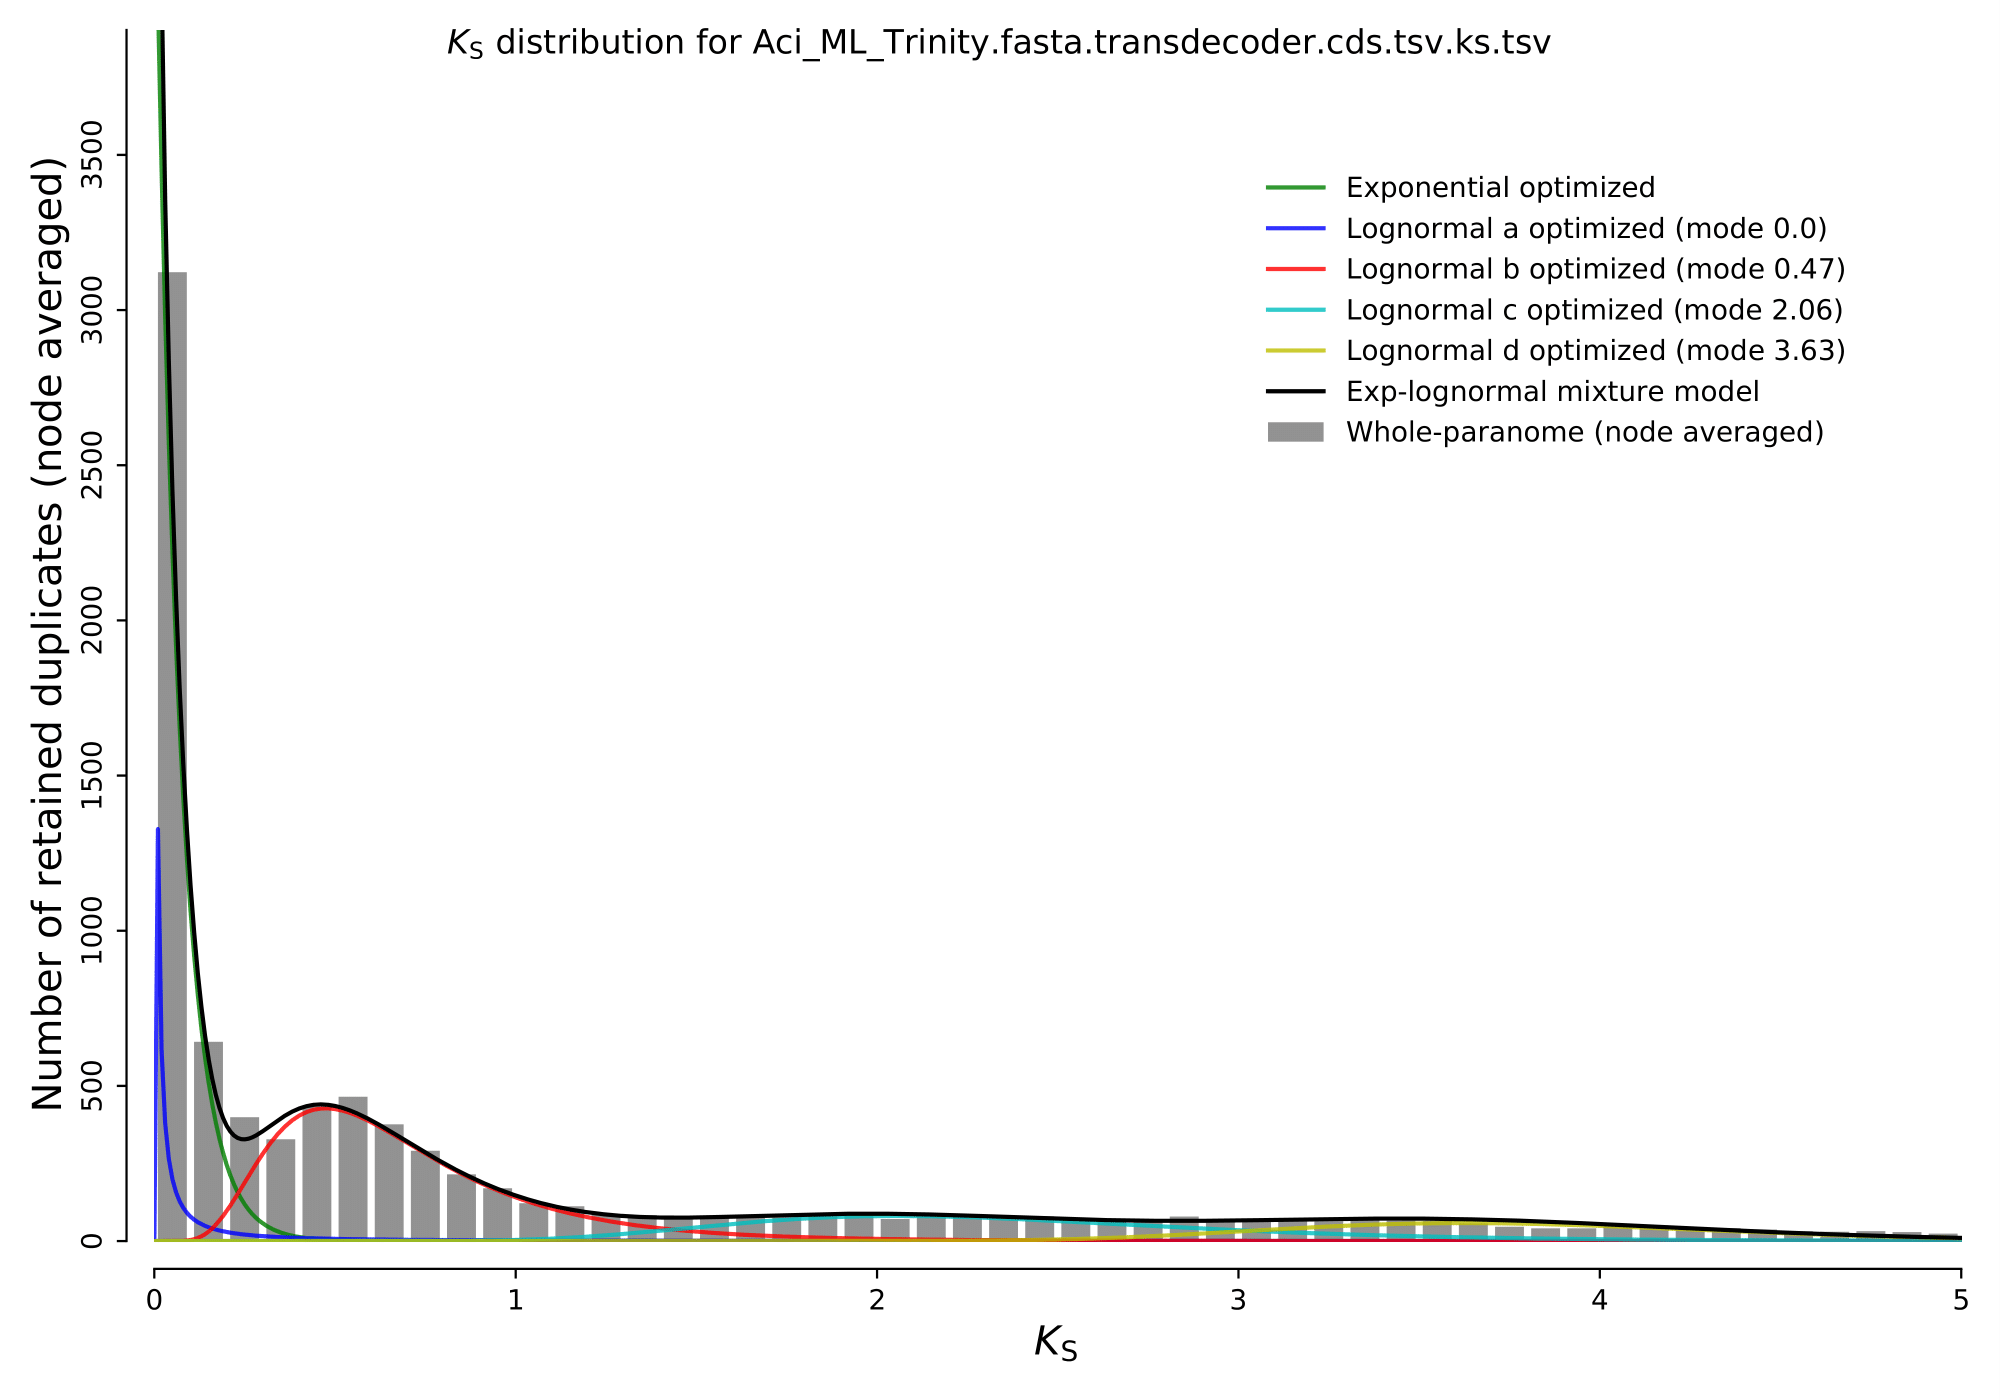
\includegraphics[width=1\linewidth]{Images/aci_ksplot} \caption{Phylogenetic tree produced from RAxML analysis on a concatenated matrix visualized using FigTree.}\label{fig:ksplot}
\end{figure}

\hypertarget{references}{%
\section{References}\label{references}}

\hypertarget{refs}{}
\begin{CSLReferences}{1}{0}
\leavevmode\vadjust pre{\hypertarget{ref-Bolger2014}{}}%
\textsc{Bolger, A.M.}, \textsc{M. Lohse}, and \textsc{B. Usadel}. 2014. \href{https://doi.org/10.1093/BIOINFORMATICS/BTU170}{Trimmomatic: A flexible trimmer for illumina sequence data}. \emph{Bioinformatics} 30: 2114--2120.

\leavevmode\vadjust pre{\hypertarget{ref-Brown2017}{}}%
\textsc{Brown, J.W.}, \textsc{J.F. Walker}, and \textsc{S.A. Smith}. 2017. \href{https://doi.org/10.1093/bioinformatics/btx063}{Phyx: Phylogenetic tools for unix}. \emph{Bioinformatics} 33: 1886--1888.

\leavevmode\vadjust pre{\hypertarget{ref-Chen2024}{}}%
\textsc{Chen, H.}, \textsc{A. Zwaenepoel}, and \textsc{Y.V. de Peer}. 2024. \href{https://doi.org/10.1093/bioinformatics/btae272}{Wgd v2: A suite of tools to uncover and date ancient polyploidy and whole-genome duplication}. \emph{Bioinformatics} 40:

\leavevmode\vadjust pre{\hypertarget{ref-Emms2019}{}}%
\textsc{Emms, D.M.}, and \textsc{S. Kelly}. 2019. \href{https://doi.org/10.1186/s13059-019-1832-y}{OrthoFinder: Phylogenetic orthology inference for comparative genomics}. \emph{Genome Biology} 20:

\leavevmode\vadjust pre{\hypertarget{ref-Faircloth2016}{}}%
\textsc{Faircloth, B.C.} 2016. \href{https://doi.org/10.1093/bioinformatics/btv646}{PHYLUCE is a software package for the analysis of conserved genomic loci}. \emph{Bioinformatics} 32: 786--788.

\leavevmode\vadjust pre{\hypertarget{ref-Grabherr2011}{}}%
\textsc{Grabherr, M.G.}, \textsc{B.J. Haas}, \textsc{M. Yassour}, \textsc{J.Z. Levin}, \textsc{D.A. Thompson}, \textsc{I. Amit}, \textsc{X. Adiconis}, et al. 2011. \href{https://doi.org/10.1038/nbt.1883}{Full-length transcriptome assembly from RNA-seq data without a reference genome}. \emph{Nature Biotechnology} 29: 644--652.

\leavevmode\vadjust pre{\hypertarget{ref-Jin2020}{}}%
\textsc{Jin, J.J.}, \textsc{W.B. Yu}, \textsc{J.B. Yang}, \textsc{Y. Song}, \textsc{C.W. Depamphilis}, \textsc{T.S. Yi}, and \textsc{D.Z. Li}. 2020. GetOrganelle: A fast and versatile toolkit for accurate de novo assembly of organelle genomes. \emph{Genome Biology} 21: 1--31. Available at: \url{https://genomebiology.biomedcentral.com/articles/10.1186/s13059-020-02154-5}.

\leavevmode\vadjust pre{\hypertarget{ref-Katoh2013}{}}%
\textsc{Katoh, K.}, and \textsc{D.M. Standley}. 2013. MAFFT multiple sequence alignment software version 7: Improvements in performance and usability. \emph{Molecular Biology and Evolution} 30: 772--780. Available at: \href{/pmc/articles/PMC3603318/\%20/pmc/articles/PMC3603318/?report=abstract\%20https://www.ncbi.nlm.nih.gov/pmc/articles/PMC3603318/}{/pmc/articles/PMC3603318/ /pmc/articles/PMC3603318/?report=abstract https://www.ncbi.nlm.nih.gov/pmc/articles/PMC3603318/}.

\leavevmode\vadjust pre{\hypertarget{ref-Lanfear2016}{}}%
\textsc{Lanfear, R.}, \textsc{P.B. Frandsen}, \textsc{A.M. Wright}, \textsc{T. Senfeld}, and \textsc{B. Calcott}. 2016. \href{https://doi.org/10.1093/molbev/msw260}{PartitionFinder 2: New methods for selecting partitioned models of evolution for molecular and morphological phylogenetic analyses}. \emph{Molecular Biology and Evolution}msw260.

\leavevmode\vadjust pre{\hypertarget{ref-Minh2020}{}}%
\textsc{Minh, B.Q.}, \textsc{H.A. Schmidt}, \textsc{O. Chernomor}, \textsc{D. Schrempf}, \textsc{M.D. Woodhams}, \textsc{A.V. Haeseler}, \textsc{R. Lanfear}, and \textsc{E. Teeling}. 2020. IQ-TREE 2: New models and efficient methods for phylogenetic inference in the genomic era. \emph{Molecular Biology and Evolution} 37: 1530--1534. Available at: \url{https://dx.doi.org/10.1093/molbev/msaa015}.

\leavevmode\vadjust pre{\hypertarget{ref-Pease2018}{}}%
\textsc{Pease, J.B.}, \textsc{J.W. Brown}, \textsc{J.F. Walker}, \textsc{C.E. Hinchliff}, and \textsc{S.A. Smith}. 2018. \href{https://doi.org/10.1002/ajb2.1016}{Quartet sampling distinguishes lack of support from conflicting support in the green plant tree of life}. \emph{American Journal of Botany} 105: 385--403.

\leavevmode\vadjust pre{\hypertarget{ref-Prjibelski2020}{}}%
\textsc{Prjibelski, A.}, \textsc{D. Antipov}, \textsc{D. Meleshko}, \textsc{A. Lapidus}, and \textsc{A. Korobeynikov}. 2020. \href{https://doi.org/10.1002/cpbi.102}{Using SPAdes de novo assembler}. \emph{Current Protocols in Bioinformatics} 70:

\leavevmode\vadjust pre{\hypertarget{ref-Smith2015}{}}%
\textsc{Smith, S.A.}, \textsc{M.J. Moore}, \textsc{J.W. Brown}, and \textsc{Y. Yang}. 2015. \href{https://doi.org/10.1186/s12862-015-0423-0}{Analysis of phylogenomic datasets reveals conflict, concordance, and gene duplications with examples from animals and plants}. \emph{BMC Evolutionary Biology} 15: 150.

\leavevmode\vadjust pre{\hypertarget{ref-Stamatakis2014}{}}%
\textsc{Stamatakis, A.} 2014. RAxML version 8: A tool for phylogenetic analysis and post-analysis of large phylogenies. \emph{Bioinformatics} 30: 1312--1313. Available at: \url{https://academic.oup.com/bioinformatics/article-lookup/doi/10.1093/bioinformatics/btu033}.

\leavevmode\vadjust pre{\hypertarget{ref-Tillich2017}{}}%
\textsc{Tillich, M.}, \textsc{P. Lehwark}, \textsc{T. Pellizzer}, \textsc{E. Ulbricht-Jones}, \textsc{A. Fischer}, \textsc{R. Bock}, and \textsc{S. Greiner}. 2017. GeSeq- versatile and accurate annotation of organelle genomes. \emph{Nucleic Acids Research} 45:

\leavevmode\vadjust pre{\hypertarget{ref-Wick2015}{}}%
\textsc{Wick, R.R.}, \textsc{M.B. Schultz}, \textsc{J. Zobel}, and \textsc{K.E. Holt}. 2015. \href{https://doi.org/10.1093/bioinformatics/btv383}{Bandage: Interactive visualization of de novo genome assemblies}. \emph{Bioinformatics} 31: 3350--3352.

\leavevmode\vadjust pre{\hypertarget{ref-Zhang2018}{}}%
\textsc{Zhang, C.}, \textsc{M. Rabiee}, \textsc{E. Sayyari}, and \textsc{S. Mirarab}. 2018. ASTRAL-III: Polynomial time species tree reconstruction from partially resolved gene trees. \emph{BMC Bioinformatics} 19: 15--30. Available at: \url{https://bmcbioinformatics.biomedcentral.com/articles/10.1186/s12859-018-2129-y}.

\end{CSLReferences}

\hypertarget{appendix-1}{%
\section{Appendix 1}\label{appendix-1}}

Citations of all R packages used to generate this report.

{[}1{]} J. Allaire, Y. Xie, C. Dervieux, et al.~\emph{rmarkdown: Dynamic
Documents for R}. R package version 2.29. 2024.
\url{https://github.com/rstudio/rmarkdown}.

{[}2{]} H. Bengtsson. \emph{R.methodsS3: S3 Methods Simplified}. R package
version 1.8.2. 2022. \url{https://github.com/HenrikBengtsson/R.methodsS3}.

{[}3{]} H. Bengtsson. \emph{R.oo: R Object-Oriented Programming with or without
References}. R package version 1.27.0. 2024.
\url{https://github.com/HenrikBengtsson/R.oo}.

{[}4{]} H. Bengtsson. \emph{R.utils: Various Programming Utilities}. R package
version 2.12.3. 2023. \url{https://henrikbengtsson.github.io/R.utils/}.

{[}5{]} H. Bengtsson. ``The R.oo package - Object-Oriented Programming with
References Using Standard R Code''. In: \emph{Proceedings of the 3rd
International Workshop on Distributed Statistical Computing (DSC
2003)}. Ed. by K. Hornik, F. Leisch and A. Zeileis. Vienna, Austria,
Mar.~2003.
\url{https://www.r-project.org/conferences/DSC-2003/Proceedings/Bengtsson.pdf}.

{[}6{]} H. Bengtsson. ``The R.oo package - Object-Oriented Programming with
References Using Standard R Code''. In: \emph{Proceedings of the 3rd
International Workshop on Distributed Statistical Computing (DSC
2003)}. Ed. by K. Hornik, F. Leisch and A. Zeileis. Vienna, Austria,
Mar.~2003.
\url{https://www.r-project.org/conferences/DSC-2003/Proceedings/Bengtsson.pdf}.

{[}7{]} C. Boettiger. \emph{knitcitations: Citations for Knitr Markdown Files}.
R package version 1.0.12. 2021.
\url{https://github.com/cboettig/knitcitations}.

{[}8{]} D. Charif and J. Lobry. ``SeqinR 1.0-2: a contributed package to the
R project for statistical computing devoted to biological sequences
retrieval and analysis.'' In: \emph{Structural approaches to sequence
evolution: Molecules, networks, populations}. Ed. by U. Bastolla, M.
Porto, H. Roman and M. Vendruscolo. Biological and Medical Physics,
Biomedical Engineering. ISBN : 978-3-540-35305-8. New York: Springer
Verlag, 2007, pp.~207-232.

{[}9{]} D. Charif and J. R. Lobry. \emph{seqinr: Biological Sequences Retrieval
and Analysis}. R package version 4.2-36. 2023.
\url{https://seqinr.r-forge.r-project.org/}.

{[}10{]} J. Cheng, B. Schloerke, B. Karambelkar, et al.~\emph{leaflet: Create
Interactive Web Maps with the JavaScript Leaflet Library}. R package
version 2.2.2. 2024. \url{https://rstudio.github.io/leaflet/}.

{[}11{]} M. C. Koohafkan. \emph{kfigr: Integrated Code Chunk Anchoring and
Referencing for R Markdown Documents}. R package version 1.2.1. 2021.
\url{https://github.com/mkoohafkan/kfigr}.

{[}12{]} J. Ooms. \emph{magick: Advanced Graphics and Image-Processing in R}. R
package version 2.8.5. 2024. \url{https://docs.ropensci.org/magick/}.

{[}13{]} R Core Team. \emph{R: A Language and Environment for Statistical
Computing}. R Foundation for Statistical Computing. Vienna, Austria,
2023. \url{https://www.R-project.org/}.

{[}14{]} H. Wickham. \emph{ggplot2: Elegant Graphics for Data Analysis}.
Springer-Verlag New York, 2016. ISBN: 978-3-319-24277-4.
\url{https://ggplot2.tidyverse.org}.

{[}15{]} H. Wickham, J. Bryan, M. Barrett, et al.~\emph{usethis: Automate
Package and Project Setup}. R package version 3.1.0. 2024.
\url{https://usethis.r-lib.org}.

{[}16{]} H. Wickham, W. Chang, L. Henry, et al.~\emph{ggplot2: Create Elegant
Data Visualisations Using the Grammar of Graphics}. R package version
3.5.1. 2024. \url{https://ggplot2.tidyverse.org}.

{[}17{]} H. Wickham, R. François, L. Henry, et al.~\emph{dplyr: A Grammar of
Data Manipulation}. R package version 1.1.4. 2023.
\url{https://dplyr.tidyverse.org}.

{[}18{]} H. Wickham, J. Hester, W. Chang, et al.~\emph{devtools: Tools to Make
Developing R Packages Easier}. R package version 2.4.5. 2022.
\url{https://devtools.r-lib.org/}.

{[}19{]} D. Winter. \emph{pafr: Read, Manipulate and Visualize Pairwise mApping
Format Data}. R package version 0.0.2. 2020.
\url{https://dwinter.github.io/pafr/}.

{[}20{]} Y. Xie. \emph{bookdown: Authoring Books and Technical Documents with R
Markdown}. Boca Raton, Florida: Chapman and Hall/CRC, 2016. ISBN:
978-1138700109. \url{https://bookdown.org/yihui/bookdown}.

{[}21{]} Y. Xie. \emph{bookdown: Authoring Books and Technical Documents with R
Markdown}. R package version 0.41. 2024.
\url{https://github.com/rstudio/bookdown}.

{[}22{]} Y. Xie. \emph{Dynamic Documents with R and knitr}. 2nd. ISBN
978-1498716963. Boca Raton, Florida: Chapman and Hall/CRC, 2015.
\url{https://yihui.org/knitr/}.

{[}23{]} Y. Xie. \emph{formatR: Format R Code Automatically}. R package version
1.14. 2023. \url{https://github.com/yihui/formatR}.

{[}24{]} Y. Xie. ``knitr: A Comprehensive Tool for Reproducible Research in
R''. In: \emph{Implementing Reproducible Computational Research}. Ed. by V.
Stodden, F. Leisch and R. D. Peng. ISBN 978-1466561595. Chapman and
Hall/CRC, 2014.

{[}25{]} Y. Xie. \emph{knitr: A General-Purpose Package for Dynamic Report
Generation in R}. R package version 1.49. 2024.
\url{https://yihui.org/knitr/}.

{[}26{]} Y. Xie and J. Allaire. \emph{tufte: Tufte's Styles for R Markdown
Documents}. R package version 0.13. 2023.
\url{https://github.com/rstudio/tufte}.

{[}27{]} Y. Xie, J. Allaire, and G. Grolemund. \emph{R Markdown: The Definitive
Guide}. Boca Raton, Florida: Chapman and Hall/CRC, 2018. ISBN:
9781138359338. \url{https://bookdown.org/yihui/rmarkdown}.

{[}28{]} Y. Xie, C. Dervieux, and E. Riederer. \emph{R Markdown Cookbook}. Boca
Raton, Florida: Chapman and Hall/CRC, 2020. ISBN: 9780367563837.
\url{https://bookdown.org/yihui/rmarkdown-cookbook}.

{[}29{]} H. Zhu. \emph{kableExtra: Construct Complex Table with kable and Pipe
Syntax}. R package version 1.4.0. 2024.
\url{http://haozhu233.github.io/kableExtra/}.

\end{document}
